\documentclass[times, utf8, diplomski]{fer}
\usepackage{booktabs}
\usepackage{listings}

\begin{document}

% TODO: Navedite broj rada.
\thesisnumber{000}

\title{Nezamjenjivi tokeni temeljeni na Cardano lancu blokova}

\author{Sven Skender}

\maketitle

\izvornik

\zahvala{Duboko sam zahvalan svom mentoru, čije su znanje i iskustvo oblikovali moj rast i razvoj tijekom naše suradnje. Također bih želio izraziti svoju iskrenu zahvalnost svojoj zaručnici, čija je vjera u mene i podrška bili beskrajni izvor snage i ohrabrenja. Mojoj obitelji, koja je uvijek postavljala pitanje "Jesi li položio?" nakon samo dva tjedna od početka akademske godine, duboko sam zahvalan na kontinuiranoj motivaciji i vjeri u moje sposobnosti. Na kraju, želim izraziti svoju iskrenu zahvalnost svima koji su bili uz mene i pružili podršku kada mi je bila najpotrebnija.}

\tableofcontents

\chapter{Uvod}

Lanac blokova (engl. \emph{blockchain}) je temeljna tehnologija proizašla iz područja digitalnih valuta. Izvorno je bila prisutna samo u svijetu financijskih transakcija te pokretala kripto valutu Bitcoin, ali je promijenila svoj doseg i utjecala na različite sektore, mijenjajući način na koji se informacije i transakcije bilježe i provjeravaju. Tradicionalni sustavi vođenja zapisa i obrade transakcija dugo su se oslanjali na centralizirane posrednike kao što su banke, vlade i institucije treće strane. Međutim, ove centralizirane strukture podložne su ljudskim pogreškama, manipulacijama i zlonamjernim napadima. Lanac blokova, s druge strane, uvodi promjenu paradigme omogućujući distribuiranoj mreži sudionika da postignu konsenzus i održavaju zajedničku knjigu bez potrebe za posrednicima.

Na svojoj najosnovnijoj razini, lanac blokova čini nepromjenjivi i sekvencijalni lanac blokova, od kojih svaki sadrži niz provjerenih i vremenski označenih transakcija. Ovaj se lanac kontinuirano ažurira i replicira na više računala ili čvorova unutar mreže. Decentralizirana priroda sustava osigurava da niti jedan entitet nema potpunu kontrolu nad cijelim sustavom, čime se smanjuje rizik od manipulacije i povećava transparentnost. Implikacije lanca blokova protežu se daleko izvan područja financija, obuhvaćajući različite sektore, uključujući upravljanje opskrbnim lancem, zdravstvo, državne službe i prava intelektualnog vlasništva.

Jedna od mogućih primjena nalazi se i u humanitarnom razminiranju. Humanitarno razminiranje igra ključnu ulogu u postkonfliktnoj obnovi jer prisutnost mina i neeksplodiranih  sredstava predstavlja ozbiljnu prijetnju civilima i infrastrukturi. Proces protuminskog djelovanja uključuje prikupljanje podataka iz različitih izvora, uključujući daljinska istraživanja, stručno znanje o protuminskom djelovanju, formalne i neformalne povijesne zapise, kao i intervjue sa stanovništvom, bivšim borcima i očevicima. Kako nove informacije postaju dostupne ili se situacija na terenu razvija, nalazi istraživanja zahtijevaju periodična ažuriranja, a tako se pojavljuje i problem pouzdanosti podataka i skladištenja. Lanac blokova se tako pokazuje kao odličan sustav koji bi mogao trajno riješiti problem pouzdanosti podataka i nepovjerenja među više dionika. 

\chapter{Koncept tokenizacije na lancu blokova}

Kada je riječ o pohrani podataka o minama i neeksplodiranih ubojitim sredstvima, lokacijama i dodatnim metapodacima, lanac blokova pruža robusno rješenje. Tokenizacijom ovih informacija na lancu, svako eksplozivno sredstvo može se predstaviti kao jedinstvena digitalna imovina, omogućujući precizno praćenje i upravljanje. Decentralizirana priroda lanca blokova osigurava da se podaci distribuiraju na više čvorova, što ih čini otpornim na neovlašteno mijenjanje pa se time onemogućava skrivanje i brisanje podataka. Ova transparentnost i nepromjenjivost donose značajne prednosti, uključujući povećanu odgovornost, sljedivost i povjerenje u podatke. Uz lanac blokova, dionici mogu pouzdano pristupiti i provjeriti informacije povezane s minama, smanjujući rizik od slučajnih eksplozija, pomažući u naporima razminiranja i poboljšavajući opće sigurnosne standarde.

\section{Opis lanca blokova}

Lanac blokova je revolucionarna tehnologija koja iz temelja mijenja način na koji se podaci pohranjuju i upravljaju njima \cite{antonopoulos2014mastering}. U svojoj srži, lanac blokova je decentralizirana i distribuirana digitalna knjiga koja bilježi transakcije ili informacije na više računala, poznatih kao čvorovi \cite{antonopoulos2018mastering}. Ova decentralizirana priroda eliminira potrebu za središnjim tijelom, poput banke ili vlade, za provjeru i autentifikaciju transakcija. Umjesto toga, povjerenje se uspostavlja pomoću algoritama konsenzusa i kriptografskih tehnika. U lancu blokova, svaka transakcija ili dio informacije grupirani su u blok. Ti se blokovi zatim međusobno povezuju u kronološki i nepromjenjivi lanac, tvoreći potpuni lanac blokova \cite{larimer2013transactions}. Svaki blok ima svoj sažetak (engl. \emph{hash}) koji proizlazi iz svih informacija pohranjenih u tom bloku te pokazuje na prethodni blok kako je vidljivo na dijagramu \ref{fig:containers-vs-vms-diagram}. Podaci pohranjeni unutar blokova zaštićeni su pomoću naprednih kriptografskih algoritama, što čini ekstremno teškim za bilo koga da promijeni informacije ili same blokove, a da ne bude otkriven \cite{buterin2013proof}.

Jedna od ključnih značajki ove tehnologije je njezina transparentnost. Svaki sudionik u mreži ima pristup kopiji cijelog lanca, čime se osigurava da su sve transakcije i promjene podataka vidljive svima. Ova transparentnost promiče povjerenje i odgovornost, budući da se svaka zlonamjerna aktivnost ili pokušaj manipulacije može lako prepoznati i odbiti od strane mreže \cite{buterin2013ethereum}. Tehnologija omogućuje i poboljšanu sigurnost kroz mehanizme konsenzusa. Ovi mehanizmi osiguravaju da se svi čvorovi u mreži slažu oko valjanosti transakcija prije nego što se dodaju u lanac \cite{zohar2015bitcoin}. Taj se dogovor postiže različitim algoritmima konsenzusa, kao što su dokaz o radu (engl. \emph{proof of work}) ili dokaz o udjelu (engl. \emph{proof of stake}), koji zahtijevaju od sudionika da osiguraju računalnu snagu ili ulože vlastitu kripto valutu (engl. \emph{cryptocurrency}) za provjeru valjanosti transakcija.

\begin{figure}[htb]
\centering
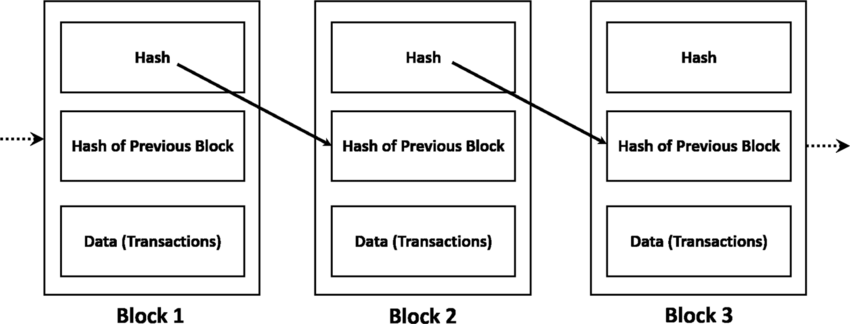
\includegraphics[width=\linewidth]{img/Simplified-diagram-of-a-blockchain.png}
\caption{Pojednostavljeni dijagram lanca blokova \cite{articlesimplifieddiagram}}
\label{fig:diagram-of-a-blockchain}
\end{figure}

Iskorištavanjem ovih temeljnih načela, ova tehnologija može se primijeniti na različite industrije i slučajeve upotrebe, uključujući upravljanje podacima o minama i neeksplodiranim sredstvima. Osigurava integritet i pouzdanost podataka sigurnim pohranjivanjem relevantnih informacija u nepromjenjivu i transparentnu glavnu knjigu. Decentralizirana priroda lanca blokova olakšava suradnju među dionicima, što dovodi do poboljšane raspodjele resursa, smanjenog dupliciranja napora i boljeg donošenja odluka u operacijama razminiranja. Štoviše, mogućnost provjere koju pruža lanac blokova povećava povjerenje u informacije i omogućuje prepoznavanje potencijalnih nedosljednosti u procesu otkrivanja mina.

\section{Svojstvo zamjenjivosti unutar tokenizacije}

Tokenizacija je proces pretvaranja imovine iz stvarnog svijeta ili digitalne imovine u tokene koji se mogu pohranjivati i prenositi na lancu blokova \cite{buterin2014daos}. Tokeni, u kontekstu lanca blokova, digitalni su prikazi imovine ili prava. Mogu se stvarati, posjedovati i prenositi, pružajući sigurnu i transparentnu metodu predstavljanja vrijednosti. Tokeni mogu predstavljati širok raspon imovine, uključujući fizičku imovinu poput nekretnina i robe, kao i nematerijalnu imovinu poput intelektualnog vlasništva, bodova vjernosti, prava pristupa određenim uslugama, sudjelovanju u procesima upravljanja itd. Vrijednost tokena obično se izvodi iz temeljne imovine ili prava koja predstavlja \cite{buterin2014daos}.

Kripto valuta je, s druge strane, specifična vrsta digitalne imovine koja služi kao sredstvo razmjene, baš kao i tradicionalne valute poput američkog dolara ili eura \cite{zohar2015bitcoin}. Glavna razlika između tokena i kripto valuta leži u njihovoj funkcionalnosti i namjeni. Dok su kripto valute poput Bitcoina \footnote{https://bitcoin.org/en/}, Ethera \footnote{https://ethereum.org/en/} i Ade \footnote{https://cardano.org/} osmišljene primarno kao mediji razmjene ili pohrane vrijednosti, tokeni mogu predstavljati mnogo širi raspon imovine i imaju specifične slučajeve upotrebe unutar ekosustava lanca blokova. Kripto valute funkcioniraju kao samostalne digitalne valute koje se mogu koristiti za razne digitalne transakcije te često rade na vlastitim lancima blokova te imaju vlastita pravila i protokole. S druge strane, tokeni se oslanjaju na postojeće platforme, kao što su Ethereum ili Cardano, za stvaranje i njihov rad. Kako se obično grade na temeljima postojećih infrastruktura, nasljeđuju njihovu sigurnost, skalabilnost i mehanizme konsenzusa. Tokeni tako nude veću fleksibilnost i prilagodbu u usporedbi s kripto valutama.

\subsection{Zamjenjivi tokeni i primjena}

Zamjenjivi tokeni (engl. \emph{fungible token}) su vrsta tokena koji su međusobno zamjenjivi i identični. Svaka jedinica zamjenjivog tokena ima istu vrijednost kao i bilo koja druga jedinica te se na tom principu mogu razmjenjivati \cite{bauer2022erc}. Klasičan primjer zamjenjivih tokena su kripto valute poput Bitcoina, Ethera ili Ade. Na primjer, ako se jedan Bitcoin zamijeni za drugi, vrijednost ostaje ista.

Zamjenjivi tokeni nalaze široku primjenu u raznim aplikacijama za decentralizirano financiranje. U aplikacijama za decentralizirano financiranje (engl. \emph{decentralized finance}, \emph{DeFi}) tokeni koji su vezani za vrijednost fiksne valute poput američkog dolara, pružaju stabilnost i obično se koriste za trgovanje \cite{schar2021decentralized}. Kao što je u stvarnom svijetu moguće zamijeniti bilo koju novčanicu jednog američkog dolara za bilo koju drugu, tako je i s tokenima koji predstavljaju vrijednost fiksne valute. Na taj način korisnici mogu trgovati tokeniziranim američkim dolarima na lancu blokova. Decentralizirani financijski protokoli tako koriste zamjenjive tokene za omogućavanje pozajmljivanja, uzgoja prinosa i drugih financijskih usluga, gdje korisnici mogu osigurati likvidnost i zaraditi kamate.

\subsection{Nezamjenjivi tokeni i primjena}

Nasuprot tome, nezamjenjivi tokeni (engl. \emph{non-fungible token}, \emph{NFT}) predstavljaju jedinstvenu digitalnu imovinu koja je nedjeljiva i razlikuje se jedna od druge \cite{wang2021non}. Svaki nezamjenjivi token posjeduje određeni identifikator koji ga izdvaja i daje mu inherentnu vrijednost. Za razliku od zamjenjivih tokena, nezamjenjivi tokeni se ne mogu izravno razmjenjivati na bazi jedan-na-jedan zbog svojih jedinstvenih karakteristika. Nezamjenjivi tokeni su posljednjih godina privukli značajnu pozornost, prvenstveno u domenama digitalne umjetnosti, kolekcionarstva i igara \cite{ante2022non}.

Nezamjenjivi tokeni su revolucionirali svijet umjetnosti omogućivši umjetnicima da tokeniziraju svoje kreacije i prodaju ih izravno kolekcionarima \cite{ante2022non}. Umjetnici mogu priložiti meta podatke svojim nezamjenjivi tokenima, pružajući dokaz o vlasništvu, autentičnosti i porijeklu. Ovo je otvorilo nove puteve za umjetnike da dopru do globalne publike, dobiju poštenu naknadu za svoj rad i zadrže kontrolu nad svojim intelektualnim vlasništvom. Pojavila su se tržišta nezamjenjivi tokena na kojima kolekcionari mogu kupovati, prodavati i trgovati digitalnim umjetninama, stvarajući svoj ekosustav za digitalne umjetnosti \cite{ante2022nona}. Štoviše, nezamjenjivi tokeni su pronašli korist i u industriji igara. Mogu predstavljati predmete u igri, likove ili virtualnu zemlju. Igrači mogu posjedovati ovu digitalnu imovinu, trgovati njome s drugim igračima, pa čak i koristiti je na više platformi za igranje.

Osim umjetnosti i igara, nezamjenjivi tokeni imaju potencijalne primjene i u područjima kao što su izdavanje ulaznica, virtualne nekretnine, prava intelektualnog vlasništva, upravljanje opskrbnim lancem itd. K tome, mogu poslužiti kao odlično sredstvo za pohranjivanje jedinstvenih geoprostornih informacija na kojima se nalaze točke od interesa u javnu i decentraliziranu bazu podataka. Tako je moguće pohranjivati lokacije raznih kampova, izvora pitke vode, SOS telefona, nalazišta rijetkih ptica, eksplozivnih i drugih opasnih naprava u bazu podataka koja ima ugrađen mehanizam za dokazivanje vlasništva, autentičnosti i jedinstvenosti.

\chapter{Aplikacija za nezamjenjive tokene (ANT)}

U sklopu ovog rada razvijena je aplikacija za kreiranje nezamjenjivih tokena na lancu blokova (ANT). Aplikacija služi kao posrednik između raznih aplikacija koje se mogu koristiti u procesu humanitarnoga razminiranja za obradu i skladištenje podataka te samog lanca blokova koji omogućava sigurnost, transparentnost i povjerljivost. Prikaz arhitekture, upute za instalaciju i korištenje sustava bit će detaljno opisane u sljedećem poglavlju. U ovom poglavlju bit će opisano istraživanje tehnologija korištenih za razvoj i implementaciju samog programskog rješenja. Bit će navedeni i objašnjeni razni alati, razvojni okviri i platforme koje će biti korištene. Prvo će biti osvijetljene temeljne tehnologije, kao što su poslužiteljske aplikacije, virtualizacija te kontejnerizacija aplikacija. Nadalje, bit će razjašnjeni napredni okviri i biblioteke koji se koriste za implementaciju rješenja te opisana Cardano platforma na kojoj cijela ideja i počiva.

\section{Poslužiteljska aplikacija}

Poslužiteljska aplikacija je program dizajniran za pružanje usluge ili resursa klijentskim aplikacijama ili uređajima. Radi na poslužitelju i odgovara na zahtjeve klijenata preko mreže. Poslužiteljske aplikacije obrađuju zadatke kao što su pohranjivanje podataka, obrada, komunikacija ili omogućavanje pristupa zajedničkim resursima. Slijede arhitekturu klijent-poslužitelj, gdje poslužitelj osluškuje dolazne klijentske zahtjeve i u skladu s tim ih obrađuje. Poslužiteljske aplikacije ključne su za omogućavanje komunikacije, suradnje i isporuke različitih usluga u umreženim okruženjima. U ovom rješenju, poslužiteljska aplikacija prima zahtjeve od drugih klijentskih aplikacija te ih  na odgovarajući način obrađuje i prosljeđuje na Cardano čvor.

\subsection{Izvršno okruženje}

Node.js \footnote{https://nodejs.org/en} je otvoreno, brzo i višeplatformsko izvršno okruženje za izvršavanje JavaScript koda. Node.js je JavaScript runtime izgrađen na V8 JavaScript engine-u, koji je razvio Google i koristi se u web preglednicima kao što je Google Chrome. Node.js omogućuje izvršavanje JavaScript koda izvan web preglednika, na poslužitelju ili na lokalnom računalu. To znači da razvojni inženjeri mogu koristiti JavaScript za pisanje poslužiteljske logike, rukovanje mrežnim zahtjevima, upravljanje datotekama, pristup bazama podataka i mnoge druge zadatke. Node.js je popularan izbor za razvoj pozadinskog sloja zbog svoje jedinstvene kombinacije prednosti. Prije svega, koristi JavaScript, široko prihvaćeni jezik kojim se pojednostavljuje razvojni proces. Također je važna i njegova sposobnost učinkovitog rukovanja asinkronim I/O operacijama bez blokiranja. To znači da Node.js može rukovati s višestrukim istodobnim vezama bez blokiranja izvođenja drugih operacija.

I/O model bez blokiranja, zajedno s V8 JavaScript engine-om, omogućuje visoko učinkovito izvršavanje koda. Ova arhitektura vođena događajima čini je posebno prikladnom za razvoj aplikacija u stvarnom vremenu, sustava za razgovor i drugih usluga gdje su odziv i skalabilnost ključni. Sve od navedenoga čini Node.js izvrsnim izborom za aplikacije koje zahtijevaju rukovanje velikim brojem istodobnih zahtjeva, kao što su API-ji i mikroservisi. Node.js može podnijeti veliku količinu istodobnih veza uz nisku potrošnju resursa. Štoviše, Node.js aplikacije mogu se lako vodoravno skalirati dodavanjem više poslužitelja za raspodjelu radnog opterećenja, omogućujući besprijekoran rast kako se potražnja korisnika povećava.

Node.js aplikacije mogu se implementirati na različitim platformama i uslugama u oblaku, što omogućuje fleksibilnost u odabiru infrastrukture. Podržava popularne platforme u oblaku kao što su AWS, Microsoft Azure i Google Cloud Platform-e, što olakšava posluživanje i skaliranje aplikacija u oblaku. Nadalje, Node.js ima koristi od opsežnog npm ekosustava. Node Package Manager (npm) je repozitorij paketa koji nudi golemu kolekciju biblioteka i modula otvorenog koda, što nevjerojatno olakšava integraciju postojećih rješenja u nove aplikacije. Node.js nudi izvrsnu podršku za rad s bazama podataka. Pruža razne biblioteke i module za interakciju s relacijskim (npr. MySQL, PostgreSQL) i NoSQL (npr. MongoDB, Redis) bazama podataka, omogućujući besprijekornu integraciju i učinkovito upravljanje podacima.

\subsection{Razvojni okvir}

Express.js \footnote{https://expressjs.com/} široko je prihvaćen okvir za izradu poslužiteljskih aplikacija izgrađen na temelju Node.js-a, pružajući robustan skup alata i značajki za izgradnju učinkovitih i skalabilnih rješenja. Jedan od glavnih razloga za korištenje Express.js-a je njegova jednostavnost i minimalistički pristup. Nudi laganu strukturu koja omogućuje veću fleksibilnost i kontrolu nad arhitekturom aplikacija. Ideja razvoja je sljedeća: počni s malim i modularnim, postupno dodajući nove komponente i funkcionalnosti kako se projekt širi.

Express.js pruža jednostavan i intuitivan API koji olakšava definiranje ruta, rukovanje zahtjevima i upravljanje međuprogramima. Također ima bogat ekosustav modula, koji omogućuju dodavanje funkcionalnosti kao što su provjera autentičnosti, zapisivanje događaja i rukovanje pogreškama. Express.js promiče mogućnost ponovne upotrebe koda kroz svoj modularni dizajn, omogućujući organizaciju koda u zasebne module i komponente za višekratnu upotrebu. Takav modularni pristup olakšava održavanje i proširivanje aplikacije tijekom vremena. 

S Express.js-om, moguće je izgraditi API-je, web usluge, pa čak i potpune web aplikacije. Pruža robusnu podršku za razvoj RESTful API-ja, što ga čini idealnim izborom za stvaranje pozadinskih usluga koje trebaju komunicirati s klijentima. Skalabilnost Express.js je još jedna prednost. Može učinkovito rukovati velikim brojem istodobnih veza, što ga čini prikladnim za aplikacije s velikim prometom ili zahtjevima u stvarnom vremenu. Express.js kompatibilan je i s različitim bazama podataka, SQL i NoSQL, omogućujući odabir baze podataka koja najbolje odgovara zahtjevima aplikacije.

Budući da Express.js pruža arhitekturu temeljenu na međuprogramima, omogućuje jednostavno dodavanje, uklanjanje ili modificiranje komponenti međuprograma kako bi se prilagodilo ponašanje aplikacije. Međuprogramski sustav je dobro osmišljen i intuitivan te omogućuje ulančavanje višestrukih međuprogramskih funkcija za obradu zahtjeva i odgovora. Takav sustav ulančavanja olakšava rad s HTTP protokolima i izvođenje uobičajenih operacija kao što je analiziranje tijela zahtjeva, rukovanje zaglavljima i postavljanje kodova odgovora. Kako se mijenjaju zahtjevi aplikacija, moguće je jednostavno dodavati nove međuprograme bez potrebe za promjenom postojećih modula i programskog koda.

\section{Cardano lanac blokova}

Cardano lanac blokova je decentralizirana platforma s dokazom o udjelu treće generacije i dom je kripto valute Ada \cite{brunjes2020utxo}. To je prva takva platforma koja se razvila iz znanstvene filozofije i pristupa koji je prvenstveno usmjeren na istraživanje. Platforma Cardano dizajnirana je od temelja i potvrđena od strane vodeće kombinacije vrhunskih inženjera i akademskih stručnjaka u područjima tehnologije lanaca blokova i kriptografije \cite{kerber2019ouroboros}. Snažan fokus je na održivosti, skalabilnosti i transparentnosti. Projekt je potpuno otvorenog koda koji ima za cilj isporučiti pravednu i otpornu infrastrukturu za financijske i društvene aplikacije na globalnoj razini. Jedan od primarnih ciljeva je pružiti pouzdane, sigurne financijske usluge onim ljudima koji trenutno nemaju pristup takvim uslugama, najviše u zemljama u razvoju.

Cardano je dizajniran sa sigurnošću kao jednim od temeljnih načela. Napisan je u funkcionalnom programskom jeziku Haskell u kojemu se potiče izgradnja sustava korištenjem čistih funkcija, što dovodi do dizajna u kojem se komponente mogu jednostavno testirati u izolaciji. Nadalje, napredne značajke programskog jezika Haskell omogućuju korištenje metoda za osiguravanje ispravnosti koda, kao što je temeljenje implementacije na formalnim i izvršnim specifikacijama, opsežno testiranje temeljeno na svojstvima i izvođenje testova u simulaciji \cite{lamela2018marlowe}. Takav pristup je posebno važan u razvoju financijskih instrumenata. Cardano platforma za pametne ugovore (engl. \emph{smart contract}) nastoji pružiti naprednije značajke od bilo kojeg prethodno razvijenog protokola i služiti kao stabilna i sigurna platforma za razvoj decentraliziranih aplikacija.

\subsection{Mehanizam konsenzusa}

Dokaz o udjelu vrsta je mehanizma konsenzusa ili protokola koji koristi količinu udjela koja se drži u sustavu za određivanje konsenzusa \cite{king2012ppcoin}. Konsenzusni protokol je ono što kontrolira zakone i parametre koji upravljaju ponašanjem lanca blokova. Konsenzus je time zapravo skup pravila kojih se pridržava svaki sudionik decentralizirane mreže. Budući da lance blokova ne kontrolira nijedno središnje tijelo, koristi se protokol konsenzusa kako bi se sudionicima distribuirane mreže omogućilo da se dogovore o povijesti mreže spremljenoj na lancu blokova, kako bi se postigao konsenzus o tome što se dogodilo i nastavilo iz jednog izvora istine.

Cardano je izgrađen na konsenzusnom protokolu Ouroboros i prvi je protokol koji je razvijen kroz recenzirana istraživanja \cite{kiayias2017ouroboros}. U središtu protokola su skupovi uloga, pouzdani čvorovi poslužitelji koje vodi operater tog uloga na koje drugi vlasnici kripto valute Ada mogu delegirati svoj ulog. Skupovi uloga koriste se kako bi se osiguralo da svi mogu sudjelovati u protokolu, bez obzira na tehničko iskustvo ili mogućnosti za održavanje čvora u radu. Ovi skupovi udjela usmjereni su na održavanje i drže kombinirane udjele različitih dionika u jednom entitetu. Nasuprot tome, dokaz o radu je sinkroni protokol koji potiče rudare da se natječu tko će prvi riješiti probleme unutar bloka. Sustav nagrađivanja koristi se za poticanje ovog rješavanja problema. Međutim, ovaj pristup ima svoju cijenu, s povećanom potrošnjom električne energije i duljim vremenskim rasponima za rješavanje problema unutar lanca.

Jedna od ključnih značajki dokaza o udjelu je da kako se broj korisnika povećava, povećava se i mogućnost održavanja glavne knjige. To znači veću šansu za proizvodnju novih blokova koji se mogu dodati u lanac. Kreator novog bloka bira se na temelju kombinacije slučajnog odabira i određivanja njegovog uloga, odnosno bogatstva koje posjeduje. Vrsta izbora vođe događa se unutar lanca. Unutar protokola za dokaz udjela sudionici akumuliraju naknade za transakcije i na taj način povećavaju svoje bogatstvo kako vrijeme prolazi. Ovaj pristup potiče stalan i stabilan rast lanca blokova i smanjuje slučajeve zaustavljenih transakcija koje mogu spriječiti rast lanca i onemogućavanje provođenja transakcija. 

Cardano ima cilj smanjiti centralizaciju te aktivno radi protiv ekonomskih poticaja koji bi vodili sustav prema centralizaciji. Čim postoje skupovi uloga, postoji i ekonomski poticaj da ti fondovi rastu, stoga je važno učiniti manje privlačnim da skup uloga postane prevelik \cite{kerber2019ouroboros}. Isplativije je imati mali broj velikih fondova nego veliki broj malih fondova. Cardano je dizajniran da radi protiv ekonomskih poticaja gdje veliki fondovi dominiraju sustavom, čineći manje privlačnim da neki fond postane prevelik. To je postignuto promjenom formule nagrađivanja. U naivnom sustavu, ukupne nagrade za skup bile bi proporcionalne njegovom ulogu, pa što je on veći, to bolje. S druge strane, ako skup privuče više uloga od određenog praga k, njegova nagrada više se neće povećavati. Dakle, ako svatko djeluje u vlastitom interesu kako bi maksimizirao svoje nagrade, onda se očekuje k skupova otprilike jednake veličine.

\subsection{Model nepotrošenog izlaza transakcije}

Cardano, poput Bitcoin lanca blokova, je temeljen na nepotrošenom izlazu transakcije (engl. \emph{unspent transaction output}, \emph{UTXO}). U takvom modelu, transakcija ima ulaze i izlaze, gdje su ulazi nepotrošeni izlazi iz prethodnih transakcija. Imovina se pohranjuje u glavnoj knjizi u nepotrošenim izlazima, a ne u računima \cite{wood2014ethereum, buterin2013ethereum, larimer2013transactions}. Izlaz transakcije uključuje adresu i vrijednost, a potpis koji pripada adresi je ključ za otključavanje izlaza. Nakon otključavanja, izlaz se može koristiti kao ulaz. Nove transakcije troše izlaze prethodnih transakcija i proizvode nove izlaze koji se mogu potrošiti u budućim transakcijama. 

Opisani proces ilustriran je na dijagramu \ref{fig:eutxo-diagram}. Kada je izlaz otključan ulazom, lanac blokova označava otključani izlaz kao potrošen. Cardanov EUTXO (engl. \emph{extended unspent transaction output}, \emph{EUTXO}) model nudi bolju skalabilnost i privatnost, kao i pojednostavljeniju transakcijsku logiku jer se svaki nepotrošeni izlaz može potrošiti samo jednom, što provjeru transakcije čini puno jednostavnijom \cite{kerber2019ouroboros}. Tako je moguć visok stupanj paralelizma jer čvor može paralelno potvrđivati transakcije ako te transakcije ne pokušavaju potrošiti isti ulaz.

Model nudi jedinstvene prednosti u odnosu na druge modele jer uspjeh ili neuspjeh validacije transakcije ovisi samo o samoj transakciji i njezinim ulazima. Kao posljedica toga, valjanost transakcije može se provjeriti izvan lanca, prije nego što se transakcija pošalje. Transakcija može ispasti nevažeća samo ako neka druga transakcija istodobno troši ulaz koji transakcija očekuje, ali ako su svi ulazi još uvijek prisutni, transakcija će zajamčeno uspjeti. To je u suprotnosti s modelom koji se temelji na računu kakav koristi Ethereum, gdje transakcija može propasti usred izvršavanja skripte \cite{antonopoulos2018mastering}. Snažna značajka ovog modela također je da se naknade potrebne za valjanu transakciju mogu točno predvidjeti prije njezinoga objavljivanja. Ovo je jedinstvena značajka koja se ne nalazi u modelima koji se temelje na računu. Lanci blokova temeljeni na računu, poput Ethereuma, nedeterministički su, što znači da ne mogu jamčiti objavu transakcije na lanac \cite{wood2014ethereum}. Ova neizvjesnost predstavlja rizik od novčanog gubitka i neočekivano visokih naknada.

\begin{figure}[htb]
\centering
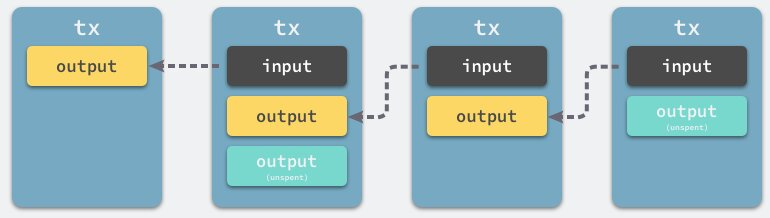
\includegraphics[width=\linewidth]{img/2018-04-05-transactions-in-utxo-model.jpg}
\caption{Prikaz transakcija koje nastaju iz nepotrošenih izlaza prethodnih transakcija \cite{blogcsdnnet}}
\label{fig:eutxo-diagram}
\end{figure}

\subsection{Izvorni tokeni}

Izvorni tokeni (engl. \emph{native token}) nova su značajka koja omogućuje transakcije više sredstava na Cardano lancu blokova. Korisnici mogu obavljati transakcije s kripto valutom Ada i neograničenim brojem korisnički definiranih tokena. Izvorna podrška nudi različite prednosti za razvojne inženjere: nema potrebe za stvaranjem pametnih ugovora za rukovanje tokenima, što uklanja sloj dodatne složenosti i potencijal za pogreške. Lanac blokova koji podržava praćenje prijenosa i vlasništva nad različitim vrstama imovine zapravo ima podršku za više sredstava. U Cardano okruženju ovu funkcionalnost pruža značajka izvornih tokena. Za vrsta lanca blokova koji ima ugrađenu podršku za praćenje vlasništva i prijenosa više od jedne vrste imovine kaže se da ima izvornu podršku. Ako platforma podržava funkcionalnost pametnih ugovora, moguće je pratiti imovinu za koju ne postoji izvorna podrška, ali to se onda postiže pomoću rješenja drugog sloja i takva vrsta podrške onda nije izvorna.

Izvorni tokeni predstavljaju određenu vrijednost i djeluju kao obračunska jedinica koja se može koristiti za plaćanja, transakcije i može se poslati na novu adresu \cite{barbiancardano}. Iako i Ada i izvorni tokeni imaju vrijednost i djeluju kao jedinica za plaćanje i transakciju, samo se Ada koristi za plaćanje naknade i dobivanje nagrada \cite{barbiancardano}. Ovo svojstvo kripto valute Ade posljedica je konstrukcije temeljnog protokola konsenzusa. Svaka adresa mora sadržavati minimalnu Ada vrijednost kako bi se mogli prenijeti drugi izvorni tokeni. Iz toga slijedi da je nemoguće stvoriti izlaze koji sadrže samo tokene. 

Broj svake vrste tokena u izlazu ne utječe na minimalnu vrijednost izlaza, ali broj vrsta tokena sadržanih u izlazu povećava tu minimalnu vrijednost. Razlog za to je taj što nazivi i ID-evi svake vrste tokena zauzimaju dodatni prostor u izlazu. Na taj način, slanje tokena na adresu uvijek uključuje i slanje minimalne vrijednosti Ada kripto valute na tu adresu. Prije prijenosa tokena, korisnici mogu koristiti komunikaciju izvan lanca kako bi pregovarali tko isporučuje potrebnu vrijednost Ada kripto valute za pokrivanje troškova transakcije.

\subsection{Politika kovanja tokena}

Politika kovanja tokena (engl. \emph{minting policy}) je skup pravila koja upravljaju kovanjem i spaljivanjem imovine na lancu blokova obuhvaćene tom politikom \cite{barbiancardano}. Smisao politike kovanja je određivanje uvjeta pod kojima se tokeni mogu kreirati (engl. \emph{mint}) ili uništiti (engl. \emph{burn}). Na primjer, pravila mogu odrediti tko ima kontrolu nad opskrbom imovinom putem kovanja i spaljivanja. Politike kovanja definiraju korisnici koji žele stvoriti novu imovinu. Na primjer, korisnik bi mogao poželjeti samo sebi dopustiti da kreira određenu vrstu tokena. To bi bilo navedeno u politici kovanja. Pridržavanje pravila kovanja provjerava čvor u trenutku obrade transakcije, pokretanjem koda ili provjerom relevantnih potpisa. Transakcije se moraju pridržavati svih pravila kovanja svih sredstava koja se transakcijom pokušavaju kovati.

Sva imovina na lancu blokova nužno ima politiku kovanja. Na primjer, politika kovanja kripto valute Ada je da se nova Ada nikada ne može kovati \cite{kerber2019ouroboros}. Sredstvo nikada ne može promijeniti svoju pridruženu politiku kovanja. Drugim riječima, postojeći tokeni ne mogu se povezati s novom politikom. Korisnici, međutim, mogu otkupiti i spaliti sve postojeće tokene i kovati nove, s novom politikom kovanja. Ako je postojeće sredstvo u glavnoj knjizi obuhvaćeno određenom politikom, onda je zajamčeno da je izvorno iskovano u skladu s tom politikom. Veza između tokena i njihovih politika kovanja je trajna iz sigurnosnih razloga, takva značajka štiti korisnike i sustav od nelegitimno iskovanih tokena. Imovina povezana s različitim politikama kovanja nikad nije zamjenjiva jedna s drugom. Ako se politika kovanja tokena promijeni kroz vrijeme, to zapravo više nije isti token, jer jednostavno ne koristi jednaku politiku kovanja, i njegova se vrijednost ne može usporediti s onom izvornog tokena.

Politike kovanja mogu biti slijedeće:

\begin{enumerate}
    \item Politika jednog izdavatelja
    \item Vremenski zaključana politika kovanja
    \item Politika jednokratnog kovanja
\end{enumerate}

Politika kovanja jednog izdavatelja određuje da samo subjekt koji posjeduje određeni skup ključeva smije kovati tokene određene grupe sredstava. Na primjer, skup ključeva navedenih u politici kovanja mora potpisati transakciju kovanja. Primjer grupe sredstava koja bi koristila politiku jednog izdavatelja bili bi tokeni koji predstavljaju bejzbol kartice. Tvrtka koja proizvodi kolekcionarske kartice objavila bi ključeve potrebne za kovanje novih bejzbol kartica. To bi značilo da se nijedan novi token ne može kovati bez potpisa te tvrtke.

Vremenski zaključana politika kovanja može se koristiti za određivanje kada se tokeni mogu kovati. Na primjer, samo u određenom vremenskom intervalu ili nakon njega ili samo prije određenog vremena. Ova vrsta politike obično se ne koristi sama. Najčešće je u kombinaciji s politikom jednog izdavatelja. Na primjer, politika može glasiti da tvrtka iz prethodnog primjera može kreirati nove tokene samo kroz sljedeće dvije godine i nakon toga više neće biti moguće kreirati nove tokene.

U politici jednokratnog kovanja, kompletan skup tokena dane grupe imovine kovan je jednom specifičnom transakcijom. To znači da više nikada neće biti kovani tokeni u toj određenoj grupi sredstava. Ova vrsta politike zahtijeva dodatnu implementaciju preko pametnih ugovora. Politika jednokratnog kovanja bila bi korisna za generiranje ulaznica za koncerte. Kapacitet dvorane u kojoj će biti koncert poznat je unaprijed tako da neće biti potrebe dopustiti da se kreira više ulaznica naknadno.

Izdavatelji tokena izdaju nove tokene i održavaju rezervu tokena u optjecaju. Jednom kada se tokeni prestanu koristiti, mogu ih uništiti u skladu s politikom kovanja. Kada se iskuje novi token, ukupna ponuda tokena za taj token se povećava, ali nema utjecaja na ponudu kripto valute Ada. Ako je radi o nezamjenjivim tokenima, ukupna ponuda je jednostavno poveća na jedan komad. Izdavatelji tokena morat će zadržati nešto novca u svojim novčanicima kako bi platili naknade za te transakcije. Proces spaljivanja tokena jednostavno uklanja te tokene iz optjecaja, a ukupna ponuda tokena se smanjuje. Proces spaljivanja je identičan za zamjenjive i nezamjenjive tokene.

\section{Kontejnerizacija programskog rješenja}

Virtualizacija (engl. \emph{virtualization}) i kontejnerizacija (engl. \emph{containerization}) su dva različita pristupa implementaciji i upravljanju softverskim aplikacijama, svaki sa svojim vlastitim skupom karakteristika i slučajeva korištenja. 

\subsection{Virtualizacija i kontejnerizacija}

Virtualizacija, koja se koristi već nekoliko desetljeća, uključuje stvaranje više virtualnih strojeva (engl. \emph{virtual machine}, \emph{VM}) na jednom fizičkom poslužitelju. Svaki virtualni stroj pokreće vlastiti operativni sustav, što omogućuje izolaciju aplikacija i resursa. Virtualizacija pruža jaku izolaciju i sigurnost između virtualnih strojeva budući da su odvojeni od temeljnog hardvera. Međutim, virtualni strojevi dolaze s određenim troškovima u smislu korištenja resursa i vremena podizanja sustava zbog potrebe za oponašanjem hardvera.

Kontejnerizacija je, s druge strane, novija tehnologija koja se pojavila s usponom Dockera \footnote{https://www.docker.com/}. Docker spremnici enkapsuliraju aplikacije i njihove ovisnosti, omogućujući im dosljedan rad u različitim računalnim okruženjima. Za razliku od virtualnih strojeva, spremnici dijele jezgru operacijskog sustava, što ih čini laganima i bržima za pokretanje. Oni nude visoku prenosivost, skalabilnost i učinkovito korištenje resursa. Kontejnerizacija se temelji na konceptu slika koje sadrže sve što je potrebno za pokretanje aplikacije, uključujući kod, biblioteke i konfiguracije.

Prije pojave kontejnerizacije, virtualizacija je bila primarna metoda koja se koristila za pokretanje više aplikacija na jednom poslužitelju \cite{combe2016docker}. Omogućila je bolju iskoristivost hardverskih resursa pokretanjem više virtualnih strojeva, od kojih svaki pokreće vlastiti skup aplikacija. Virtualizacija je olakšala konsolidaciju radnih opterećenja, omogućujući organizacijama da smanje broj fizičkih poslužitelja i s njima povezane troškove. Omogućila je i učinkovit način upravljanja složenim infrastrukturama i osigurala izolaciju između aplikacija. 

Međutim, virtualizacija je imala određene nedostatke. Zahtijevala je više resursa zbog pokretanja više operacijskih sustava i upravljanja njihovim zasebnim instancama \cite{anderson2015docker}. Virtualni strojevi su se također sporije pokretali, što ih je činilo manje prikladnim za aplikacije koje je potrebno brzo skalirati. Dodatno, troškovi i složenost upravljanja virtualnim strojevima učinili su izazovnim postizanje brze implementacije i kontrole verzija. Kontejnerizacija je riješila ta ograničenja uvođenjem lagane, skalabilne i brže alternative. Kontejneri dijele jezgru OS-a domaćina, što rezultira smanjenim opterećenjem i bržim vremenom pokretanja. Opisana usporedba može se vidjeti na slici \ref{fig:containers-vs-vms-diagram}.

\begin{figure}[htb]
\centering
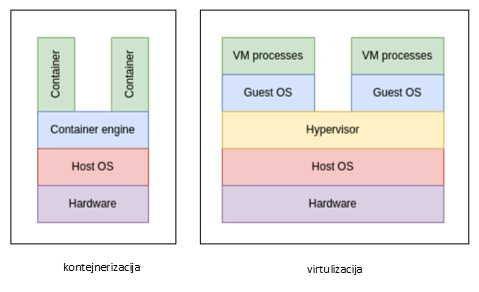
\includegraphics[width=\linewidth]{img/containers-vs-vms-diagram.png}
\caption{Razlika u arhitekturi kontejnerizacije (lijevo) i virtulizacije (desno)}
\label{fig:containers-vs-vms-diagram}
\end{figure}

Mogu se brzo osigurati i skalirati, što ih čini idealnim za moderne arhitekture mikroservisa i aplikacije u oblaku. Kontejnerizacija također pojednostavljuje implementaciju aplikacije, budući da se kontejneri mogu lako pakirati, otpremati i raditi dosljedno u različitim okruženjima, od lokalnih razvojnih strojeva do proizvodnih poslužitelja. 

U ovom programskom rješenju, kontejnerizacija je posebno zanimljiva zbog pojednostavljenja prenosivosti razvijene aplikacije između raznih okruženja i poslužitelja. Također, omogućuje brzo skaliranje aplikacije, izolaciju grešaka i pojačanu sigurnost jer je aplikacija izolirana unutar spremnika te se tako sprječava da potencijalni zlonamjerni kod utječe na druge spremnike ili na sustav domaćina.

\subsection{Docker i mikroservisi}

Docker je kontejnerska platforma otvorenog koda koja je revolucionirala način na koji se softverske aplikacije razvijaju, pakiraju i pokreću \cite{docker2020docker}. Uz Docker, aplikacije i njihove ovisnosti su enkapsulirane u lagane, prijenosne spremnike koji se mogu dosljedno izvoditi u različitim računalnim okruženjima. Spremnici se često nazivaju "lagani", što znači da dijele jezgru operacijskog sustava stroja. Spremnici pružaju samostalnu okolinu za izvođenje, uključujući kod aplikacije, biblioteke i konfiguracije, omogućujući besprijekorno i pouzdano izvođenje. 

Docker pojednostavljuje proces implementacije aplikacije eliminirajući potrebu za brigom o razlikama u temeljnoj infrastrukturi \cite{docker2020docker}. Razvojni inženjeri mogu izgraditi Docker slike koje sadrže sve potrebne komponente i ovisnosti, osiguravajući dosljedno ponašanje bez obzira na glavni sustav. Te se slike mogu dijeliti, kontrolirati verzijom i lako reproducirati, smanjujući složenost implementacije. Ova prenosivost sprječava zaključavanje usluge u oblaku ili od strane nekog drugog ponuđača usluge te nudi druge značajne prednosti kao što su izolacija grešaka i izolacija sigurnosti. Kontejnerske aplikacije su "izolirane" po tome što se ne spajaju u kopiju operacijskog sustava. Umjesto toga, Docker se instalira na operativni sustav domaćina i postaje kanal za spremnike koji dijele operacijski sustavi s drugim spremnicima na istom računalnom sustavu.

Docker omogućuje brzo skaliranje i učinkovitost resursa dopuštajući da više spremnika radi na istom glavnom računalu, učinkovito iskorištavajući dostupne resurse \cite{docker2020docker}. Spremnici se mogu brzo pokretati i gasiti, omogućujući odgovore na promjenjive zahtjeve i neprimjetno skaliranje aplikacije. Docker također promiče arhitekturu mikroservisa, gdje se složene aplikacije rastavljaju na manje, labavo povezane usluge koje se mogu neovisno razvijati, testirati i implementirati u spremnike. Nove aplikacije temeljene na oblaku mogu se izgraditi iz temelja kao kontejnerske mikroservisi, razlažući složenu aplikaciju na niz manjih specijaliziranih usluga kojima se može upravljati. Postojeće aplikacije mogu se prepakirati u spremnike koji učinkovitije koriste računalne resurse. 

Mikroservisi se prihvaćaju kao superioran pristup razvoju i upravljanju aplikacijama, u usporedbi s ranijim monolitnim modelom koji kombinira softversku aplikaciju s pridruženim korisničkim sučeljem i bazom podataka u jedinstvenu jedinicu na platformi jednog poslužitelja \cite{docker2020docker}. S primjenom mikroservisa, složena aplikacija razbijena je u niz manjih, više specijaliziranih usluga, od kojih svaka ima svoju bazu podataka i svoju poslovnu logiku. Mikroservisi zatim međusobno komuniciraju preko uobičajenih sučelja (kao što su API-ji) i REST sučelja (kao što je HTTP). Koristeći mikroservise, razvojni timovi mogu se usredotočiti na ažuriranje određenih dijelova aplikacije bez utjecaja na nju kao cjelinu.

Koncepti koji stoje iza mikroservisa i kontejnerizacije slični su budući da su obje prakse razvoja softvera koje u biti pretvaraju aplikacije u zbirke manjih usluga ili komponenti koje su prenosive, skalabilne, učinkovite i kojima je lakše upravljati. Štoviše, mikroservisi i kontejnerizacija dobro funkcioniraju kada se koriste zajedno. Spremnici pružaju laganu enkapsulaciju bilo koje aplikacije, bilo da se radi o tradicionalnom monolitu ili modularnom mikroservisu. 

Današnje komunikacije brzo se sele u oblak gdje korisnici mogu brzo i učinkovito razvijati aplikacije \cite{docker2020docker}. Aplikacije i podaci temeljeni na oblaku dostupni su s bilo kojeg uređaja povezanoga s internetom, što članovima tima omogućuje daljinski rad i u pokretu. Pružatelji usluga u oblaku (engl. \emph{cloud service provider}, \emph{CSP}) upravljaju temeljnom infrastrukturom, što organizacijama štedi troškove poslužitelja i druge opreme, a također omogućuje automatizirano mrežno sigurnosno kopiranje za dodatnu pouzdanost \cite{docker2020docker}. Infrastrukture oblaka skaliraju se na zahtjev i mogu dinamički prilagoditi računalne resurse, kapacitet i infrastrukturu kako se zahtjevi opterećenja mijenjaju. Povrh toga, CSP-ovi redovito ažuriraju ponude, dajući korisnicima stalni pristup najnovijoj inovativnoj tehnologiji.

\subsection{Komunikacija između procesa}

Komunikacija između procesa koji se izvode u različitim Docker spremnicima može se postići različitim metodama, ovisno o specifičnim zahtjevima i slučajevima korištenja. Neki od često korištenih pristupa su sljedeći:

\begin{itemize}
    \item Mrežna komunikacija: Spremnici mogu međusobno komunicirati pomoću mrežnih protokola kao što su TCP/IP ili UDP. Svakom spremniku dodijeljena je IP adresa unutar Docker mreže, što procesima unutar različitih spremnika omogućuje uspostavljanje veza i razmjenu podataka preko te iste mreže.
    \item Redovi poruka ili brokeri: Uvođenje reda poruka ili brokera, kao što je RabbitMQ, Apache Kafka ili Redis, može olakšati komunikaciju između spremnika. Spremnici mogu objavljivati poruke u redu poruka, a drugi spremnici mogu konzumirati te poruke. Ovaj asinkroni komunikacijski obrazac koristan je za odvajanje procesa i omogućavanje skalabilne komunikacije otporne na greške.
    \item Dijeljeni volumeni: Docker spremnici mogu dijeliti podatke koristeći dijeljene volumene. Zajednički volumen spojen je na više spremnika, omogućujući im čitanje i pisanje podataka na istu lokaciju na glavnom sustavu. Dijeljenjem volumena, procesi u različitim spremnicima mogu razmjenjivati datoteke ili pristupati zajedničkom izvoru podataka \ref{fig:docker-vol}.
\end{itemize}

\begin{figure}[htb]
\centering
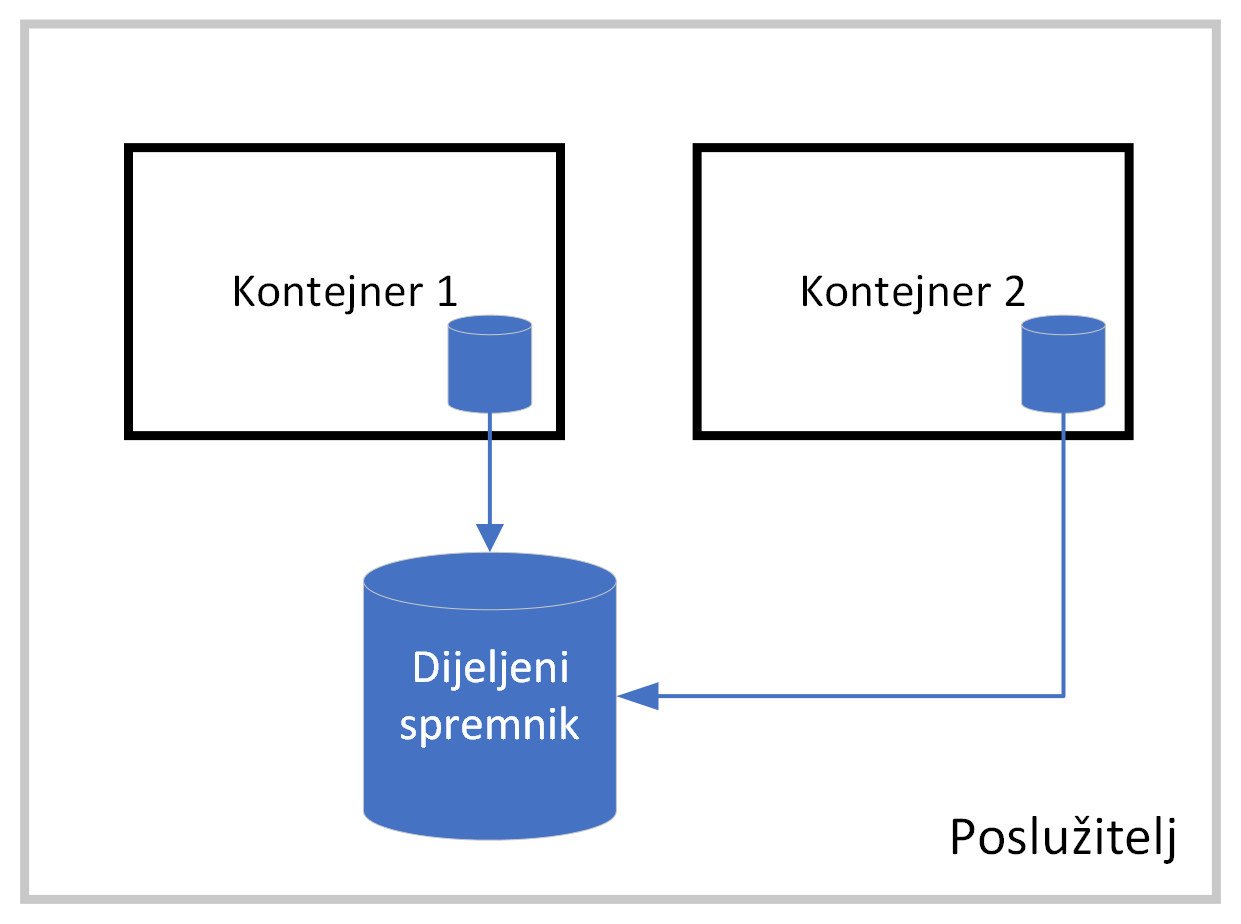
\includegraphics[width=10cm]{img/com.png}
\caption{Dijeljenje zajedničkog prostora za pohranu između Docker kontejnera}
\label{fig:docker-vol}
\end{figure}

U ovom rješenju komunikacija između Cardano čvora i razvijene aplikacije vrši se preko priključne utičnice, također poznata kao Unix domenska socket komunikacija. Takva vrsta komunikacije omogućuje procesima da uspostave komunikacijske kanale koristeći posebne socket datoteke umjesto mrežnih protokola. Kada programi žele komunicirati putem socket datoteka, obično slijede model klijent-poslužitelj. Poslužiteljski program stvara socket datoteku i veže je na određenu stazu u datotečnom sustavu. Klijentski program povezuje se s ovom datotekom utičnice pomoću putanje datoteke. Nakon što se veza uspostavi, programi mogu razmjenjivati podatke čitanjem i pisanjem u deskriptor datoteke. 

Programi prenose podatke na temelju unaprijed dogovorenoga komunikacijskog protokola, koji može biti jednostavan tekstualni protokol ili složeniji binarni protokol. Specifični format i značenje podataka određuju aplikacije uključene u komunikaciju. Komunikacija preko takve datoteke pruža lagan i učinkovit mehanizam za komunikaciju između procesa. Ostvarenje takve komunikacije realizirano je preko dijeljenog volumena između dva kontejnera. Dijeljeni volumen služi za pohranjivanje socket datoteke. Oba spremnika zatim mogu pristupiti socket datoteci preko tog spojenog volumena.

\chapter{Implementacija programskog rješenja}

Razvijeno programsko rješenje sastoji se od dvije glavne komponente: lokalnog Cardano čvora i poslužiteljske aplikacije koja stoji kao posrednik između Cardano lanca blokova i svojih klijenata. Poslužiteljska aplikacija omogućava svojim klijentima da preko HTTP protokola razmjenjuju podatke s Cardano lancem blokova. Ona translatira jednostavne zahtjeve poslane preko HTTP protokola u naredbe razumljive Cardano protokolu. Uz to, u potpunosti apstrahira kreiranje i potpisivanje transakcija te općenito svu interakciju s kripto novčanicima. Važno je napomenuti da se za klijente podrazumijeva da se radi o drugim mrežnim aplikacijama, a ne fizičkim osobama. Razvijeno programsko rješenje je zamišljeno da se koristi unutar nekog sustava te da ima dobru mrežnu i fizičku zaštitu lokacije na kojoj se nalazi jer upravlja kripto valutom i tokenima od osobite važnosti.

\section{Arhitektura programskog rješenja}

Arhitektura cjelokupnog programskog rješenja prikazana je na slici \ref{fig:arhitektura}. S lijeve strane nalazi se Cardano čvor, zapakiran u Docker kontejner. Podatci s čvora spremaju se u dijeljeni volumen, a čvor razmjenjuje poruke s javnom Cardano mrežom, odnosno lancem blokova, preko mrežnog protokola. Razvijena poslužiteljska aplikacija, također zapakirana u Docker kontejner, komunicira s lokalnim Cardano čvorom preko spomenutog dijeljenog volumena koristeći Unix priključnu utičnicu. Aplikacija svoje podatke, odnosno podatke kripto novčanika, sprema u poseban volumen samo za tu namjenu. Uz to, aplikacija prima HTTP zahtjeve od drugih servisa. Ti servisi se mogu nalaziti u drugim Docker kontejnerima ili na skroz odvojenim sustavima. Na taj način aplikacija služi kao posrednik za prenošenje zahtjeva svojih klijenata na i sa Cardano lanca blokova. 

\begin{figure}[htb]
\centering
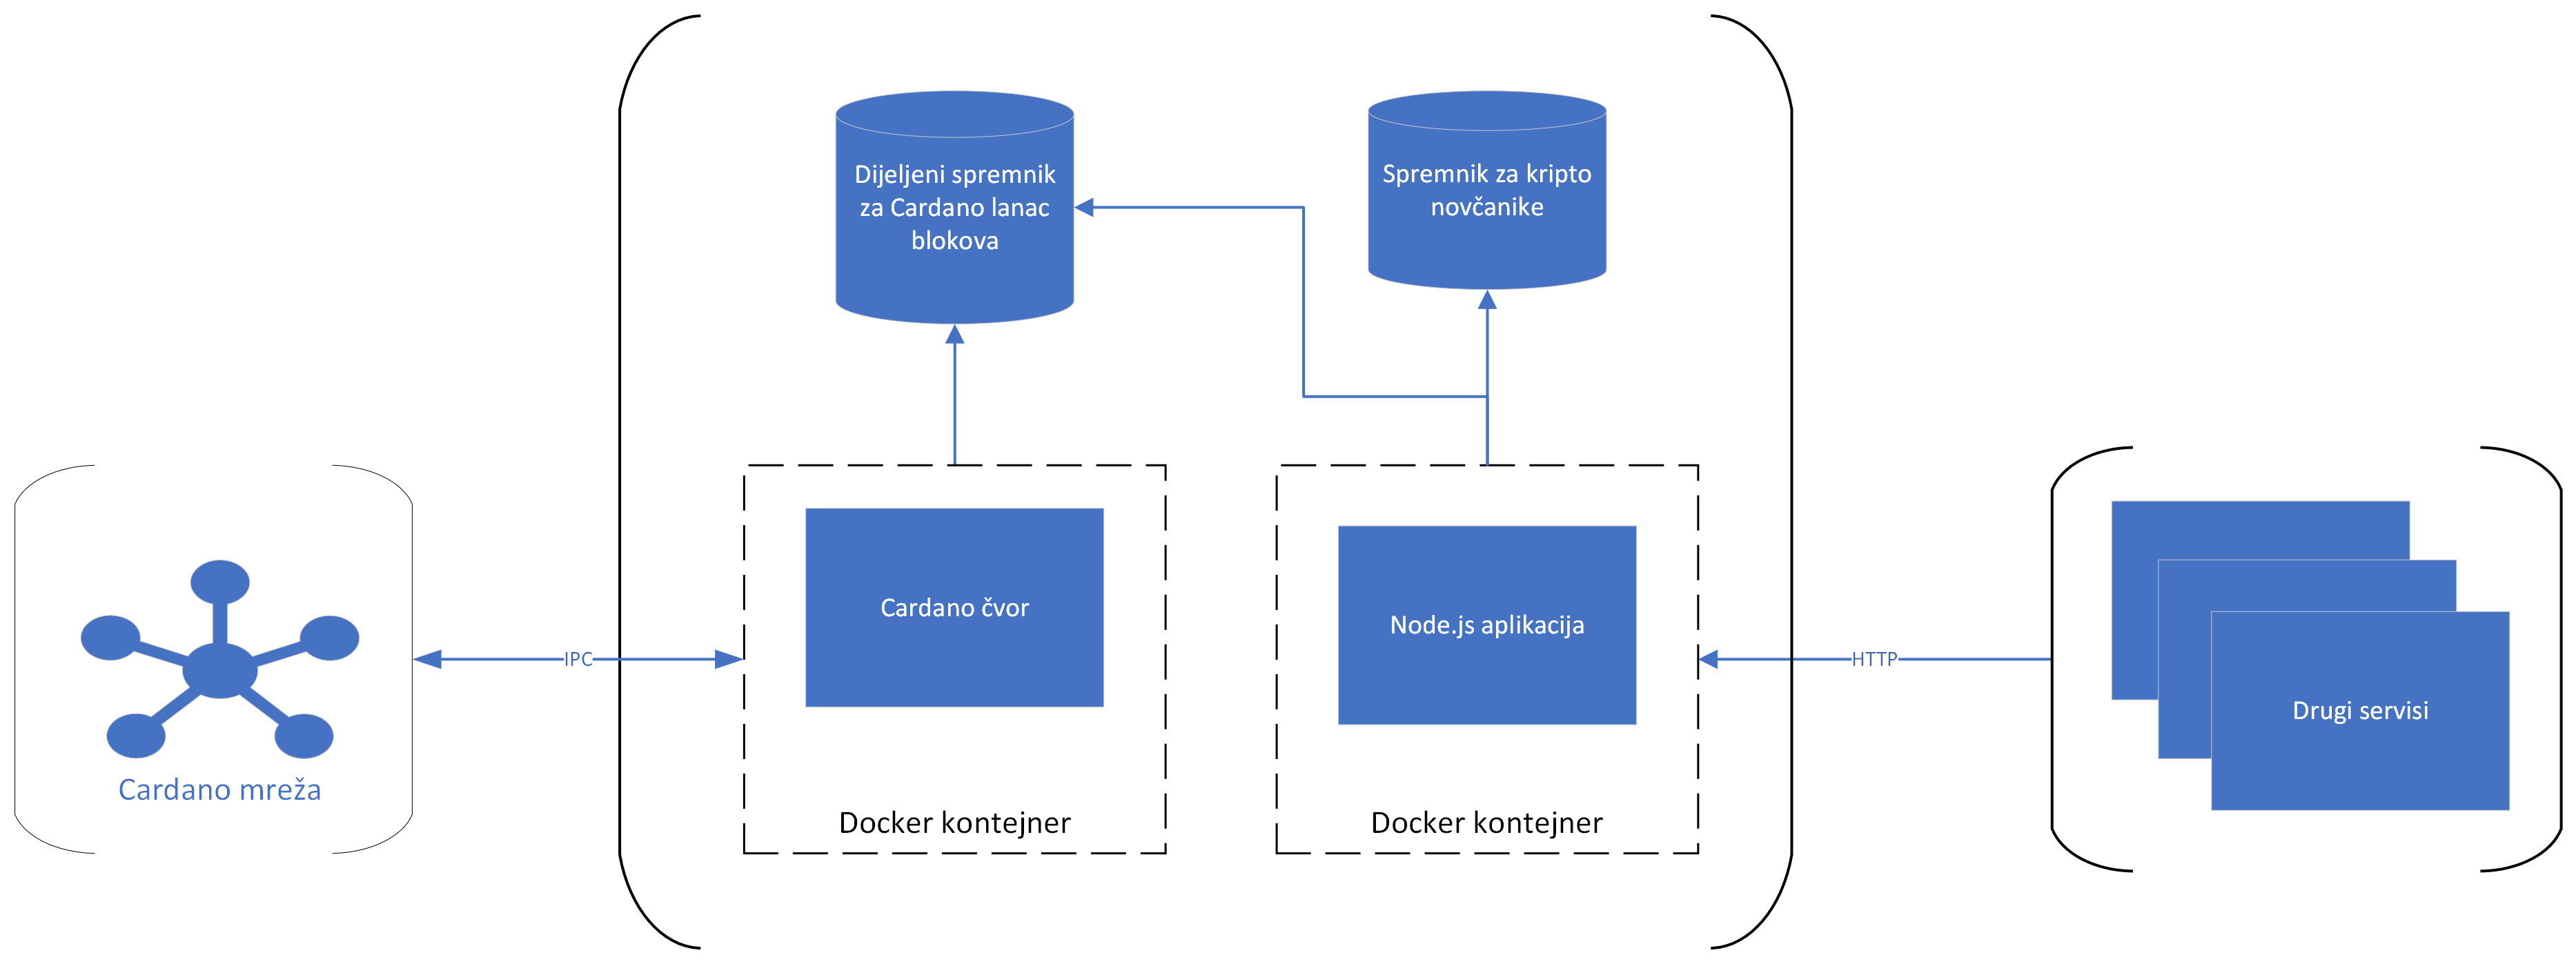
\includegraphics[width=\linewidth]{img/cardano.png}
\caption{Prikaz arhitekture programskog rješenja}
\label{fig:arhitektura}
\end{figure}

\section{Pokretanje Cardano čvora i sinkronizacija}

Kako bi se osigurala uspješna instalacija i besprijekorno izvođenje aplikacije, ključno je uzeti u obzir hardverske specifikacije sustava. Preporučeni hardverski zahtjevi pokazuju da sustav treba imati minimalno 4 gigabajta (GiB) radne memorije (RAM) i najmanje 4 procesorske jezgre. Dodatno, kapacitet pohrane od 100 gigabajta (GiB) neophodan je za rad Cardano čvora. Međutim, važno je napomenuti da će se veličina Cardano lanca blokova povećati u budućnosti, stoga je preporučljivo dodijeliti više prostora za pohranu od navedenoga minimuma. Štoviše, veća količina radne memorije značajno poboljšava brzinu sinkronizacije lanca blokova, zbog čega je dobro imati i do 16 gigabajta (GiB) RAM-a. Ispunjavanjem ili premašivanjem ovih specifikacija hardvera, korisnici mogu osigurati optimalne performanse i izbjeći moguće probleme s kompatibilnosti tijekom korištenja aplikacije.

Za pokretanje programskog rješenja potrebno je najprije instalirati Docker alat. Docker pruža platformu za pakiranje i distribuciju programskog rješenja u izoliranom okruženju, te tako omogućuje izvođenje aplikacije bez potrebe za instalacijom dodatnih paketa i ručnim namještanjem postavki sustava. Samo aplikacija i Cardano čvor su zapakirani u zasebne Docker slike koje je potrebno pokrenuti te ih potom povezati preko dijeljenog spremnika kako bi programi međusobno mogli komunicirati i razmjenjivati poruke.

Za početak je potrebno napraviti tri direktorija. Na Unix sustavima to je moguće napraviti sa sljedećom naredbom:

\begin{verbatim}
   mkdir {environment,cardano-data,wallet-data}
\end{verbatim}

U kreirane direktorije spremat će se redom sljedeće vrste datoteka: postavke mreže za Cardano čvor, Cardano lanac blokova - odnosno cijela povijest svih transakcija ikad nastalih na Cardano lancu blokova te podatci kripto novčanika.

Kako bi se Cardano čvor pravilno pokrenuo i kako bi se osiguralo da je spojen na pravu vrstu i verziju mreže, potrebno je preuzeti službenu konfiguraciju i pohraniti je u environment mapu. Pri pokretanju, Cardano će učitati konfiguraciju iz mape. U sljedećim primjerima, bit će korištena konfiguracija za testnet mrežu, točnije za pre-prod testnet vrstu mreže. Ta vrsta mreže je idealna za testiranje aplikacija na lancu blokova u uvjetima jednakima kao što su na samoj mainnet mreži, s jedinom razlikom u tome da nije potrebno trošiti pravu kripto valutu Ada pa samim time ni pravi novac. Korisnik može biti siguran da će se aplikacija koja je isprobana na pre-prod mreži ponašati jednako i u mainnet mreži.

Sve postavke za pre-prod mrežu mogu se preuzeti koristeći naredbu \texttt{curl}; kako slijedi:

\lstset{tabsize=2,breaklines=true,postbreak=\mbox{{$\hookrightarrow$}\space}}
\begin{lstlisting}
curl -O -J https://book.world.dev.cardano.org/environments/preprod/config.json
curl -O -J https://book.world.dev.cardano.org/environments/preprod/db-sync-config.json
curl -O -J https://book.world.dev.cardano.org/environments/preprod/submit-api-config.json
curl -O -J https://book.world.dev.cardano.org/environments/preprod/topology.json
curl -O -J https://book.world.dev.cardano.org/environments/preprod/byron-genesis.json
curl -O -J https://book.world.dev.cardano.org/environments/preprod/shelley-genesis.json
curl -O -J https://book.world.dev.cardano.org/environments/preprod/alonzo-genesis.json
curl -O -J https://book.world.dev.cardano.org/environments/preprod/conway-genesis.json
\end{lstlisting}

Proces za korištenje mainnet mreže je identičan, jedino je potrebno preuzeti druge konfiguracijske datoteke:

\lstset{tabsize=2,breaklines=true,postbreak=\mbox{{$\hookrightarrow$}\space}}
\begin{lstlisting}
curl -O -J https://book.world.dev.cardano.org/environments/mainnet/config.json
curl -O -J https://book.world.dev.cardano.org/environments/mainnet/db-sync-config.json
curl -O -J https://book.world.dev.cardano.org/environments/mainnet/submit-api-config.json
curl -O -J https://book.world.dev.cardano.org/environments/mainnet/topology.json
curl -O -J https://book.world.dev.cardano.org/environments/mainnet/byron-genesis.json
curl -O -J https://book.world.dev.cardano.org/environments/mainnet/shelley-genesis.json
curl -O -J https://book.world.dev.cardano.org/environments/mainnet/alonzo-genesis.json
curl -O -J https://book.world.dev.cardano.org/environments/mainnet/conway-genesis.json
\end{lstlisting}

Sada je moguće pokrenuti Cardano čvor u Docker kontejneru pomoću sljedeće naredbe:

\lstset{tabsize=2,breaklines=true,postbreak=\mbox{{$\hookrightarrow$}\space}}
\begin{lstlisting}
docker run \
    --name cardano-node \
    --volume $PWD/environment:/configuration \
    --volume $PWD/cardano-data:/opt \
    inputoutput/cardano-node run \
        --config /configuration/config.json \
        --topology /configuration/topology.json
\end{lstlisting}

Naredba pokreće Docker kontejner imena cardano-node i pomoću parametara --volume spaja konfiguraciju iz mape environment koja se nalazi u trenutnom direktoriju s mapom configuration koja se nalazi unutar Docker kontejnera. Na taj način se Cardano čvoru omogućava da pročita preuzetu konfiguraciju za spajanje na mrežu. Drugi volumen na jednak način spaja podatke s Cardano mreže u lokalnu mapu cardano-data te tako pohranjuje cijelu povijest lanca blokova na lokalni disk. Ako se nekada kasnije zatvori Docker kontejner ili ponovno pokrene poslužitelj, svi podatci ostat će spremljeni na lokalnom disku. Kada se Docker kontejner ponovno pokrene, samo će učitati već postojeće datoteke i neće biti potrebno ponovno sinkronizirati cijeli lanac blokova.

Jednom kada je Cardano čvor pokrenut, počet će sinkronizaciju s ostatkom mreže. Taj proces može potrajati od nekoliko sati do nekoliko dana, ovisno o performansama sustava i brzini interneta. Nužno je da sinkronizacija završi u potpunosti prije nego li se aplikacija može početi koristiti. Status Docker kontejnera i same sinkronizacije moguće je pratiti preko sljedeće naredbe:

\begin{verbatim}
docker ps
\end{verbatim}

koja daje ispis:

\lstset{tabsize=2,breaklines=true,postbreak=\mbox{{$\hookrightarrow$}\space}}
\begin{lstlisting}
CONTAINER ID   IMAGE                      NAMES
6625b5e6d143   inputoutput/cardano-node   cardano-node
\end{lstlisting}

i pogledom u zapise iz kontejnera:

\begin{verbatim}
docker logs -f cardano-node
\end{verbatim}

koji daje sljedeći ispis:

\lstset{tabsize=2,breaklines=true,postbreak=\mbox{{$\hookrightarrow$}\space}}
\begin{lstlisting}
CARDANO_BIND_ADDR=0.0.0.0
CARDANO_BLOCK_PRODUCER=false
CARDANO_CONFIG=/configuration/config.json
Listening on http://127.0.0.1:12798
CARDANO_DATABASE_PATH=/opt/cardano/data
CARDANO_LOG_DIR=/opt/cardano/logs
CARDANO_PORT=3001
CARDANO_SOCKET_PATH=/opt/cardano/ipc/socket
CARDANO_TOPOLOGY=/configuration/topology.json
Byron; Shelley
1.35.5
\end{lstlisting}

Iz ispisa je vidljivo koja je konfiguracija učitana, putanje na važne datoteke i utičnice, broj bloka koji se trenutno sinkronizira itd.

Nakon što je cijeli lanac blokova sinkroniziran s Cardano čvorom, u ispisu će to biti i vidljivo na sljedeći način:

\lstset{tabsize=2,breaklines=true,postbreak=\mbox{{$\hookrightarrow$}\space}}
\begin{lstlisting}
Started opening Chain DB
Started opening Immutable DB
Validating chunk no. 567 out of 567. Progress: 99.82%
Validated chunk no. 567 out of 567. Progress: 100.00%
\end{lstlisting}

Nakon ovoga koraka, moguće je preći na sljedeći korak, instalaciju i pokretanje same aplikacije.

\section{Instalacija aplikacije}

Cijela aplikacija i svi potrebni paketi spakirani su u jednu Docker sliku koja se stvara iz priloženog Dockerfile-a. Dockerfile sadrži skup instrukcija koje je potrebno pokrenuti kako bi se stvorila Docker slika u kojoj se nalazi aplikacija zajedno sa svim potrebnim komponentama. Dockerfile je prikazan u nastavku:

\lstset{tabsize=2,breaklines=true,postbreak=\mbox{{$\hookrightarrow$}\space}}
\begin{lstlisting}
FROM node:lts-slim

ARG CARDANO_VERSION=1.35.5

ENV TZ=UTC
RUN ln -snf /usr/share/zoneinfo/$TZ /etc/localtime && echo $TZ > /etc/timezone
RUN apt update && apt install --no-install-recommends -y wget

WORKDIR /opt/cardano-node
ENV CARDANO_VERSION=$CARDANO_VERSION
RUN wget --no-check-certificate \
    "https://update-cardano-mainnet.iohk.io/cardano-node-releases/cardano-node-$CARDANO_VERSION-linux.tar.gz"
RUN tar -xzf cardano-node-$CARDANO_VERSION-linux.tar.gz
RUN mv cardano-cli /usr/local/bin
WORKDIR /opt
RUN rm -rf cardano-node

WORKDIR /opt/cardano-middleware

COPY package.json .
COPY package-lock.json .

ENV NODE_ENV=production
ENV CARDANO_NODE_SOCKET_PATH=/opt/cardano/ipc/socket

RUN npm ci --omit=dev
COPY . .

VOLUME [ "priv" ]
EXPOSE 3000

CMD ["npm", "start"]
\end{lstlisting}

Na početku skripte uzima se već spremna Docker slika s instaliranom Node.js aplikacijom. Upotreba ovakve slike slijedi sve dobre sigurnosne prakse kod izgradnje novih Docker slika. U nju se preuzima binarna datoteka cardano-cli verzije 1.35.5 koja je definirana na početku kao argument za izgradnju slike. Za korištenje neke druge verzije Cardano klijenta potrebno je promijeniti varijablu \texttt{CARDANO\_VERSION}, a pri stvaranju slike bit će instalirana točna verzija. Nakon toga, pomoću \texttt{npm} naredbi instaliraju se svi potrebni paketi za produkcijsku verziju Node.js aplikacije, te se na kraju konačno pokreće poslužiteljska aplikacija.

Da bi se stvorila Docker slika naziva \texttt{cardano-middleware} iz navedenoga niza instrukcija, potrebno je pokrenuti sljedeću naredbu:

\begin{verbatim}
docker build --tag cardano-middleware:latest .
\end{verbatim}

Nakon uspješno provedene akcije, moguće je vidjet popis svih dostupnih Docker slika na sustavu pomoću sljedeće naredbe:

\lstset{tabsize=2,breaklines=true,postbreak=\mbox{{$\hookrightarrow$}\space}}
\begin{lstlisting}
docker image ls

REPOSITORY                 TAG       IMAGE ID       SIZE
cardano-middleware         latest    6b7749da8e0d   891MB
inputoutput/cardano-node   latest    bba793bf23cd   946MB
\end{lstlisting}

Jedino što je još preostalo je pokrenuti novo kreiranu Docker sliku i povezati je preko dijeljenog spremnika na drugi Docker kontejner u kojemu je pokrenut Cardano čvor. Preko tog dijeljenog spremnika vršit će se sva komunikacija između aplikacije i Cardano čvora. Drugi volumen koji se povezuje je \texttt{wallet-data} i služi za spremanje datoteka od kripto novčanika na lokalni disk. Dodatno se povezuju i vrata na kojima aplikacija sluša nadolazeće HTTP zahtjeve na vrata poslužitelja, tako da se aplikacijskom sučelju može pristupiti izravno preko vrata broj 80, što označava da se radi o standardnom HTTP protokolu. Moguće je, naravno, koristiti i neka druga dostupna vrata. Navedeno se radi sljedećom naredbom:

\lstset{tabsize=2,breaklines=true,postbreak=\mbox{{$\hookrightarrow$}\space}}
\begin{lstlisting}
docker run \
    --name cardano-middleware \
    --publish 80:3000 \
    --volume $PWD/cardano-data/cardano/ipc/socket:/opt/cardano/ipc/socket \
    --volume $PWD/wallet-data:/opt/cardano-middleware/priv \
    cardano-middleware:latest
\end{lstlisting}

Pri pokretanju Docker kontejnera vidljiv je sljedeći ispis iz aplikacije koji prikazuje verziju aplikacije i učitani profil, u ovom slučaju radi se o produkcijskom profilu. Također su vidljive i dodatne informacije, kao što su Cardano mreža na koju je aplikacija spojena te dostupni kripto novčanici. Postavke oko mreže i kripto novčanika bit će detaljno objašnjene u sljedećem poglavlju.

\lstset{tabsize=2,breaklines=true,postbreak=\mbox{{$\hookrightarrow$}\space}}
\begin{lstlisting}
> cardano-middleware@1.0.0 start
> node src/index.js

{"level":"info","message":"Connecting through /opt/cardano/ipc/socket"}
{"level":"info","message":"Connected to testnet-magic 1"}
{"level":"info","message":"Loading wallets..."}
{"level":"info","message":"Creating wallet 'Wallet1'"}
{"level":"info","message":"Created wallet 'Wallet1' successfully"}
{"level":"info","message":"Creating wallet 'Wallet2'"}
{"level":"info","message":"Created wallet 'Wallet2' successfully"}
{"level":"info","message":"Creating wallet 'Wallet3'"}
{"level":"info","message":"Created wallet 'Wallet3' successfully"}
{"level":"info","message":"App running in production environment"}
\end{lstlisting}

Kako bi se provjerilo da aplikacija uistinu radi pravilno i ima mogućnost obrade HTTP zahtjeva, može se napraviti jednostavni HTTP GET zahtjev preko \texttt{curl} naredbe:

\begin{verbatim}
curl "http://127.0.0.1/api/v1/health"
\end{verbatim}

Ako je sve ispravno pokrenuto i aplikacija je uspješno učitala sve postavke i ima mogućnost odgovora na klijentove zahtjeve, dobiva se sljedeći odgovor:

\begin{verbatim}
{"success":true,"status":"UP"}
\end{verbatim}

Navedena HTTP ruta može se koristiti kao jednostavna provjera statusa aplikacije i može se implementirati na način da i vanjski sustavi automatizirano provjeravaju status. Budući da se naredba pokreće na istom poslužitelju na kojem je i Docker kontejner pokrenut, a aplikacija sluša na vratima 80, moguće joj je pristupiti preko adrese localhost na IP adresi 127.0.0.1. Na potpuno jednak način može se pristupiti aplikaciji i preko javne IP adrese poslužitelja tako da je potrebno dobro osigurati tko sve ima mrežni pristup ovoj i ostalim rutama.

\section{Postavke aplikacije i kripto novčanika}

Sve postavke vezane za aplikaciju i kripto novčanike mogu se pronaći u \texttt{src/config.js} konfiguracijskoj datoteci. U njoj se nalaze postavke od HTTP poslužitelja pa je tako moguće promijeniti zadana vrata na kojima aplikacija sluša zahtjeve, razinu opsežnosti ispisa, konfiguracijski profil te na kraju postavke vezane za Cardano čvor. Sve postavke moguće je definirati i u \texttt{.env} datoteci iz koje će one biti učitane pri pokretanju aplikacije. U slučaju da je datoteka prazna, bit će učitane zadane postavke koje su definirane u konfiguracijskoj datoteci. Pri pokretanju aplikacije u Docker kontejneru, varijabla \texttt{NODE\_ENV} postavljena je na vrijednost \texttt{production}, vrata na vrijednost \texttt{3000}, a \texttt{LOG\_LEVEL} na razinu \texttt{debug} kako bi se i poruke najniže razine ispisivale na konzoli.

\lstset{tabsize=1,breaklines=true,postbreak=\mbox{{$\hookrightarrow$}\space}}
\begin{lstlisting}
module.exports = {
 profile: process.env.NODE_ENV || 'development',
 port: process.env.PORT || 3000,
 logger: {
  logLevel: process.env.LOG_LEVEL || 'debug',
 },
 cardano: {
  socketPath: process.env.CARDANO_NODE_SOCKET_PATH,
  network: process.env.CARDANO_NETWORK || 'testnet-magic 1',
  wallets: ['Wallet1', 'Wallet2', 'Wallet3'],
 },
};
\end{lstlisting}

Postavke vezane uz sam Cardano čvor nalaze se u odjeljku pod nazivom \texttt{cardano}. Postavka \texttt{socketPath} definira lokaciju utičnice preko koje se vrši komunikacija s Cardano čvorom. Ta postavka je u Docker kontejneru već postavljena pri pokretanju na komunikaciju preko dijeljenog spremnika tako da ju nema potrebe mijenjati. Postavka odabira mreže postavljena je na zadanu vrijednost \texttt{testnet-magic 1} i odnosi se na \texttt{pre-prod} mrežu na koju je prethodno postavljen Cardano čvor preko preuzetih konfiguracijskih datoteka. Da bi se koristila neka druga vrsta mreže potrebno je promijeniti tu vrijednost, a sve moguće vrijednosti mogu se pronaći na službenoj Cardano stranici. U tom slučaju, potrebno je pokrenuti i u potpunosti sinkronizirati Cardano čvor na željenu mrežu. Za prelazak na mainnet potrebno je varijablu \texttt{CARDANO\_NETWORK} postaviti na vrijednost \texttt{mainnet} u konfiguracijskoj ili \texttt{.env} datoteci.

Druga postavka vezana za Cardano čvor je odabir kripto novčanika. U polje \texttt{wallets} navode se imena novčanika koji se planiraju koristiti za plaćanje i potpisivanje transakcija. Minimalno jedan novčanik mora bit naveden i taj služi za potpisivanje transakcija, plaćanje naknada, a na njegovoj adresi nastaju kovani tokeni. Svi ostali novčanici mogu se koristiti isključivo za potpisivanje transakcija. Tako je na primjer moguće imati tri različite organizacije, od kojih svaka ima svoj kripto novčanik. Jedna organizacija se brine o tome da se na njenom novčaniku uvijek nalaze dostupna sredstva za plaćanje naknada, a ostale organizacije, odnosno njihovi novčanici, su tu kako bi transakcija bila važeća jer se smatra da je transakcija valjana jedino ako su se sve tri organizacije složile i potpisale tu transakciju. 

Kroz vrijeme je, naravno, moguće tu listu organizacija i proširiti dodavanjem novih kripto novčanika. U danom primjeru koda postavljena su tri zadana novčanika imena \texttt{Wallet1}, \texttt{Wallet2} i \texttt{Wallet3}. Pri pokretanju aplikacije, učitava se konfiguracija novčanika, provjerava se postoje je li već svi novčanici, te se stvaraju oni koji nedostaju. Pri inicijalnom pokretanju, kada nijedan novčanik još nije kreiran, tim procesom će oni biti stvoreni te će aplikacija započeti s radom. Primjer ispisa kod prvog pokretanja i stvaranja kripto novčanika vidljiv je ispod:

\lstset{tabsize=2,breaklines=true,postbreak=\mbox{{$\hookrightarrow$}\space}}
\begin{lstlisting}
{"level":"info","message":"Loading wallets..."}
{"level":"info","message":"Creating wallet 'Wallet1'"}
{"level":"info","message":"Created wallet 'Wallet1' successfully"}
{"level":"info","message":"Creating wallet 'Wallet2'"}
{"level":"info","message":"Created wallet 'Wallet2' successfully"}
{"level":"info","message":"Creating wallet 'Wallet3'"}
{"level":"info","message":"Created wallet 'Wallet3' successfully"}
{"level":"info","message":"App running in production environment"}
\end{lstlisting}

\section{Status i prijenos sredstava}

Pri interakciji s bilo kojom vrstom lanca blokova, pa tako i lancem blokova Cardano, potrebno je znati određene informacije o stanju čvora. Jedna od informacija je status sinkronizacije, odnosno je li čvor sinkroniziran s ostatkom mreže ili nije, koji je zadnji blok koji je primljen itd. Te informacije se dalje mogu usporediti preko raznih platformi kako bi se zaključilo radi li sve ispravno. 

Kako bi bili sigurni da je transakcija uspješno zapisana na lanac, potrebno je pogledati koliko je nastalo novih blokova otkad je transakcija zapisana u svoj blok. Ne postoji jednostavno pravilo za izračunati koliko blokova je potrebno za to, već se to radi statističkom procjenom vjerojatnosti. Ta vjerojatnost zapravo govori kolike su šanse da će trenutni lanac ostati važeći pa tako i transakcija koja je pohranjena u jedan od blokova u tom lancu. Što je više blokova u lancu, to su te šanse veće. Ukratko, svaki korisnik za sebe, ovisno o tome kako se odnosi prema riziku, mora procijeniti taj broj potrebnih blokova. Sve potrebne informacije za to mogu se dobiti preko sljedeće HTTP GET rute:

\begin{verbatim}
http://127.0.0.1/api/v1/node/info
\end{verbatim}

Ova ruta prikazuje sve informacije dohvaćene s Cardano čvora, tako da je čvor moguće nadgledati direktno kroz aplikaciju. Isto kao što je slučaj i s prethodnom rutom, ova ruta može se implementirati u vanjskom sustavu za automatiziranu provjeru statusa Cardano čvora.

\lstset{tabsize=1,breaklines=true,postbreak=\mbox{{$\hookrightarrow$}\space}}
\begin{lstlisting}
{
 "success": true,
 "data": {
  "block": 1009780,
  "epoch": 73,
  "era": "Babbage",
  "hash": "db179d9dc5fb0e33c019af23408eef1aaebf
  c7b18369d5d71e1fd3cbdf265707",
  "slot": 30112931,
  "syncProgress": "100.00"
 },
 "status": 200
}
\end{lstlisting}

Sve rute su implementirane na način da vraćaju HTTP statusni kod i logičku varijablu \texttt{success} preko koje se može doznati je li naredba uspješno izvršena u aplikaciji. Sva ostala informacijska polja nalaze se zapakirana u varijablu imena \texttt{data}.

Za prijenos sredstava na kripto novčanike i praćenje njihovog stanja, potrebno je znati adrese novčanika. HTTP GET ruta \texttt{wallet/address} vraća parove imena i pripadnih adresa svih novčanika. Obzirom da su u postavkama definirana tri novčanika, ruta vraća točno te novčanike naziva \texttt{Wallet1}, \texttt{Wallet2} i \texttt{Wallet3}. Stanje svakoga od njih vidljivo je preko rute \texttt{wallet/balance}. Početno stanje svakog novčanika je očekivano 0 Ada.

\begin{verbatim}
http://127.0.0.1/api/v1/wallet/address
\end{verbatim}

\lstset{tabsize=1,breaklines=true,postbreak=\mbox{{$\hookrightarrow$}\space}}
\begin{lstlisting}
{
"success": true,
"data": {
 "Wallet1": "addr_test1qzdf8eu7fas4u6y3jf77669sx2yrcreu7c2lkua
 6jjntalq08de9jgjqzpa9ql09jdrm4lpnxd425cq72nwgy
 nyfar6qtrjn0h",
 "Wallet2": "addr_test1qpcaffmmpsqg9e7jhf7czz9l2nucuhey6rer387
 0xs0w7y30gul
 ke0jdghshyppue3dhfvhlpqfthmhxxv32atdenmrq9s5uk6",
 "Wallet3": "addr_test1qq6gtc77hz2ucjrd8mrdhcxh950zk2lhdkuhu8m
 va2zt55s654r
 yjuy5eqgmuy6djv2379k0cx4peeflmqt600hu230svmv9nt"
},
"status": 200
}
\end{lstlisting}

\begin{verbatim}
http://127.0.0.1/api/v1/wallet/balance
\end{verbatim}

\lstset{tabsize=1,breaklines=true,postbreak=\mbox{{$\hookrightarrow$}\space}}
\begin{lstlisting}
{
 "success": true,
 "data": {
  "Wallet1": 0,
  "Wallet2": 0,
  "Wallet3": 0
 },
 "status": 200
}
\end{lstlisting}

Novčanik je moguće napuniti prijenosom sredstava s bilo kojeg drugog novčanika koji sadrži kripto valutu Ada ili direktnim prijenosom s neke od dostupnih kripto mjenjačnica. Obzirom da se ovdje radi o \texttt{pre-prod} mreži, a ne \texttt{mainnet} mreži, moguće je zatražiti testnu kripto valutu Ada od Cardano organizacije. Testna kripto valuta je u potpunosti besplatna i može se dobiti preko službene stranice \footnote{https://docs.cardano.org/cardano-testnet/tools/faucet/}. Na slici je vidljiv primjer prijenosa sredstava na prvi kripto novčanik s Cardano stranice. Odabrana mreža je Preprod Testnet i ta vrijednost odgovara postavkama u konfiguraciji.

\begin{figure}[!htb]
\centering
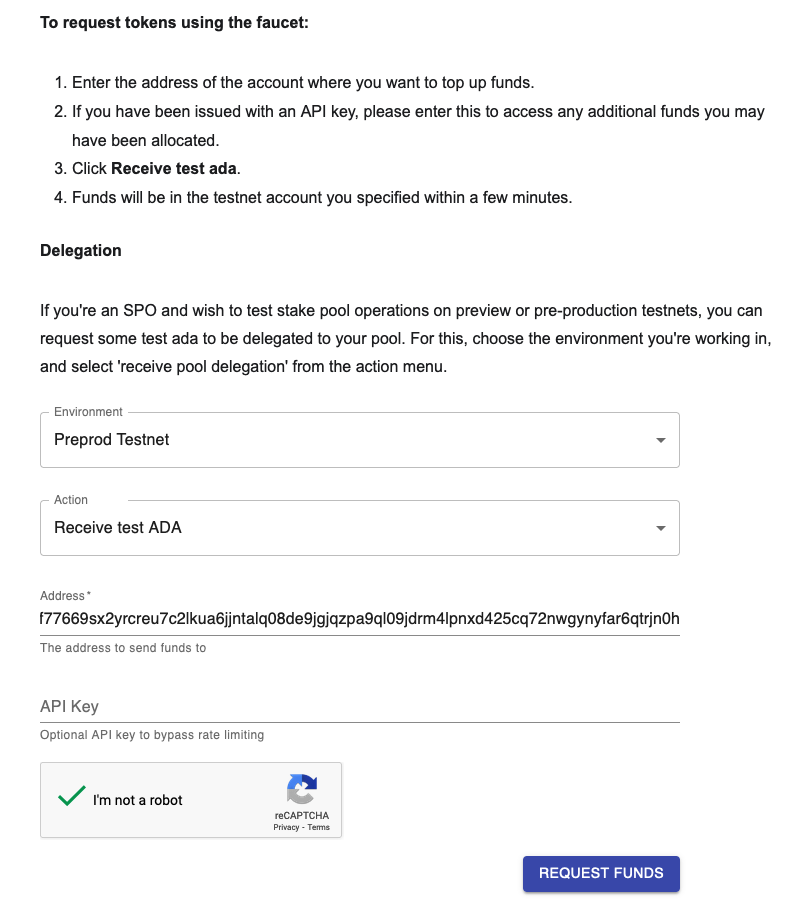
\includegraphics[width=\linewidth]{img/faucet.png}
\caption{Zatraživanje testne kripto valute Ada}
\label{fig:faucet-request}
\end{figure}

Odmah nakon slanja zahtjeva dobiva se povratna informacija da je transakcija uspješna te da je testna kripto valuta ADA poslana na adresu.

\begin{figure}[!htb]
\centering
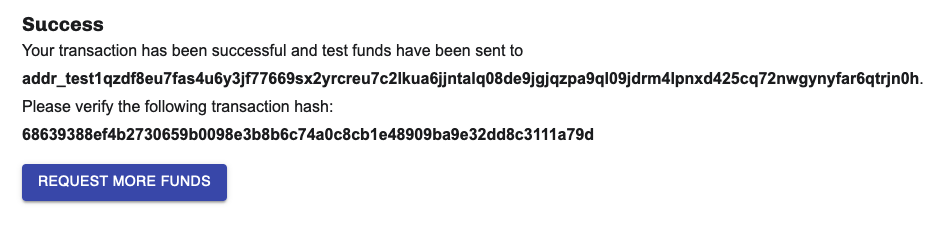
\includegraphics[width=\linewidth]{img/faucet-success.png}
\caption{Rezultat zatraživanja testne kripto valute Ada}
\label{fig:faucet-success}
\end{figure}

Nakon nekoliko minuta provjerom stanja novčanika kroz aplikaciju vidljivo je da se u prvom novčaniku sada nalazi točno 10000000000 Lovelace, što odgovara 10000 Ada (1 Ada = 1000000 Lovelace).

\lstset{tabsize=1,breaklines=true,postbreak=\mbox{{$\hookrightarrow$}\space}}
\begin{lstlisting}
{
 "success": true,
 "data": {
  "Wallet1": 10000000000,
  "Wallet2": 0,
  "Wallet3": 0
 },
 "status": 200
}
\end{lstlisting}

\section{Kovanje nezamjenjivih tokena}

Novi tokeni stvaraju se preko HTTP POST rute 

\begin{verbatim}
http://127.0.0.1/api/v1/token/mint
\end{verbatim}

U tijelo HTTP zahtjeva dodaje se JSON sa svim informacijama koje token mora sadržavati. Obavezna polja su \texttt{id} i \texttt{name}, u kojima su zapisani jedinstveni identifikator tokena i puno ime tokena. Ostala polja su opcionalna, ali ako postoje moraju biti u formatu kako slijedi:

\lstset{tabsize=1,breaklines=true,postbreak=\mbox{{$\hookrightarrow$}\space}}
\begin{lstlisting}
{
 id: 'LandMine#42',
 name: 'MRUD',
 description: 'Directed fragmentation mine',
 latitude: '45.8001454',
 longitude: '15.970733',
 files: [
  {
   name: 'File#1024',
   mediaType: 'image/png',
   src: 'QmZP1qyDSdA32763LD4hAYW6xKp59XCAig4vo9hFuqtsL6',
  },
  {
   name: 'File#1025',
   mediaType: 'image/gif',
   src: 'LiZP1qyDSdA36763LD4hAYW6xGp59XCAig4vo9hOjqtsL7',
  },
 ],
}
\end{lstlisting}

\begin{itemize}
    \item \texttt{id}: jedinstveni identifikator tokena, mora biti alfanumerički tip podatka, bez razmaka
    \item \texttt{name}: puni naziv, može sadržavati sve ASCII znakove
    \item \texttt{description}: opis, također može sadržavati sve ASCII znakove
    \item \texttt{latitude}: geografska širina na kojoj se nalazi naprava
    \item \texttt{longitude}: geografska dužina na kojoj se nalazi naprava
    \item \texttt{files}: polje datoteka koje su vezane uz napravu i njihovi izvori
    \begin{itemize}
        \item \texttt{name}: ime datoteke
        \item \texttt{mediaType}: MIME format datoteke
        \item \texttt{src}: lokacija datoteke, može biti mrežna poveznica, preporuča se da pokazuje na neku vrstu decentralizirane pohrane
    \end{itemize}
\end{itemize}

Kada poslužitelj zaprimi zahtjev za kovanjem novog tokena, prolazi kroz sljedeći skup koraka:

Kreiranje politike kovanja jednog izdavatelja koja određuje da samo subjekt koji posjeduje određeni skup ključeva smije kovati tokene ove prirode. To znači da samo kripto novčanici navedeni u konfiguraciji aplikacije mogu kreirati tokene ove vrste sada i u budućnosti.

\lstset{tabsize=1,breaklines=true,postbreak=\mbox{{$\hookrightarrow$}\space}}
\begin{lstlisting}
{
"scripts": [
 {
  "keyHash": "f67ccae63c95cc854058c0adf0e4743
  e3d23f4cfb51b7e0d49aabbf8",
  "type": "sig"
 },
 {
  "keyHash": "6bf4c457421c553fdb3b8b2bb2257729
  e2c08904ce8753d53c8e6fc0",
  "type": "sig"
 },
 {
  "keyHash": "e609d7795ef62e54ed4d15524a66be5f
  de9768e2c204c82ad58376f2",
  "type": "sig"
 }
],
"type": "all"
}
\end{lstlisting}

Kreiranje jedinstvenog identifikatora tokena iz heksadekadske vrijednosti varijable \texttt{id} i jedinstvene politike kovanja.

\begin{verbatim}
11ddf8ef671b9dba8b1d7ba65c696e8730594c617f1969f4bcf666f6
.
4c616e644d696e65233432
\end{verbatim}

\lstset{tabsize=1,breaklines=true,postbreak=\mbox{{$\hookrightarrow$}\space}}
\begin{lstlisting}
function createAssetId(assetName, policyId) {
 logger.info('Creating asset id from name and policy...');

 const assetNameHex = Buffer.from(assetName).toString('hex');
 const assetId = `${policyId}.${assetNameHex}`;

 logger.info(assetId);

 return assetId;
}
\end{lstlisting}

Obrada meta podatka iz tijela zahtjeva u format koji je moguće spremiti na lanac blokova, zajedno s kreiranim identifikatorom i politikom kovanja. Rezultat ove obrade je potpuno važeći JSON objekt koji definira strukturu izvornog nezamjenjivog tokena na Cardano lancu blokova. Takva vrsta tokena ima kodno ime 721 koje na Cardano lancu blokova govori da se radi o nezamjenjivom tokenu te omogućava Cardano protokolu da izvršava sve daljnje operacije s tim tokenom.

\lstset{tabsize=1,breaklines=true,postbreak=\mbox{{$\hookrightarrow$}\space}}
\begin{lstlisting}
{
 "721": {
  "11ddf8ef671b9dba8b1d7ba65c696e87305
  94c617f1969f4bcf666f6": {
   "LandMine#42": {
    "name": "MRUD",
    "description": "Directed fragmentation mine",
    "files": [
      {
       "mediaType": "image/png",
       "name": "File#1024",
       "src": "QmZP1qyDSdA32763LD4hAYW6xKp
       59XCAig4vo9hFuqtsL6"
      },
      {
       "mediaType": "image/gif",
       "name": "File#1025",
       "src": "LiZP1qyDSdA36763LD4hAYW6xGp5
       9XCAig4vo9hOjqtsL7"
      }
    ],
    "latitude": "45.8001454",
    "longitude": "15.970733"
   }
  }
 }
}
\end{lstlisting}

Kreiranje transakcije radi se na način da se uzmu prethodno ne-potrošene transakcije iz primarnoga kripto novčanika (primarni kripto novčanik je prvi novčanik u popisu kripto novčanika u konfiguracijskoj datoteci) i upotrijebe se kao ulazne transakcije u novoj transakciji. Iz njih se dobije potrebna količina kripto valute Ada za plaćanje naknada kod slanja transakcije u mrežu. Izlazne transakcije iz nove transakcije čine ne-potrošeni ostatak ulaznih transakcija i jedan novi token količine jedan. Količina jedan odgovara tome da se radi upravo o nezamjenjivom tokenu. U varijabli \texttt{mint} koristi se prethodno kreirana skripta politike kovanja, a u varijabli \texttt{metadata} sve ostale informacije o novom tokenu. Varijabla \texttt{witnessCount} označava broj svjedoka transakcije, odnosno broj novčanika koji tu transakciju potpisuju.

Zadano je da svi dostupni novčanici potpisuju transakciju pa je tako taj broj postavljen na vrijednost duljine polja u kojemu su ti kripto novčanici navedeni. Iz tih informacija preko Cardano čvora kreira se nova transakcija. Na kraju je potrebno još samo ostaviti dovoljno kripto valute Ada za plaćanje naknada mreži. To se može napraviti na način da se dobije trenutno potrebna minimalna naknada na mreži s Cardano čvora te se onda ta količina oduzme od nepotrošenih ulaza u ovu transkciju. Cijeli proces rezultira time da izlazi iz nove transakcije sadrže jedan novi nezamjenjivi token i sve prethodno ne-potrošene transakcije izuzev male količine kripto valute Ada koja će biti potrošena na plaćanje naknade mreži. Naposljetku se iz tako formirane transakcije ponovno kreira transakcija preko Cardano čvora u svom izvornom formatu te se vraća kao rezultat opisane funkcije.

\lstset{tabsize=1,breaklines=true,postbreak=\mbox{{$\hookrightarrow$}\space}}
\begin{lstlisting}
function buildTransaction(assetId, mintScript, metadata) {
 logger.info('Building transaction...');

 const tx = {
  txIn: primaryWallet.balance().utxo,
  txOut: [
   {
    address: primaryWallet.paymentAddr,
    value: { ...primaryWallet.balance().value, [assetId]: 1 },
   },
  ],
  mint: [{ action: 'mint', quantity: 1, asset: assetId, script: mintScript }],
  metadata,
  witnessCount: wallets.length,
 };

 logger.info(tx);

 const rawTx = cardano.transactionBuildRaw(tx);
 const fee = cardano.transactionCalculateMinFee({
  ...tx,
  txBody: rawTx,
 });

 tx.txOut[0].value.lovelace -= fee;

 logger.info(tx);

 return cardano.transactionBuildRaw({ ...tx, fee });
}
\end{lstlisting}

Rezultat kreiranja transakcije:

\lstset{tabsize=1,breaklines=true,postbreak=\mbox{{$\hookrightarrow$}\space}}
\begin{lstlisting}
{
 "metadata": {
  "721": {
   "11ddf8ef671b9dba8b1d7ba65c696e8730594c617f1969
   f4bcf666f6": {
    "LandMine#42": {
     "description": "Directed fragmentation mine",
     "files": [
      {
       "mediaType": "image/png",
       "name": "File#1024",
       "src": "QmZP1qyDSdA32763LD4hAYW6xKp59XCAig4
       vo9hFuqtsL6"
      },
      {
       "mediaType": "image/gif",
       "name": "File#1025",
       "src": "LiZP1qyDSdA36763LD4hAYW6xGp59XCAig4
       vo9hOjqtsL7"
      }
     ],
     "latitude": "45.8001454",
     "longitude": "15.970733",
     "name": "MRUD"
    }
   }
  }
 },
 "mint": [
  {
   "action": "mint",
   "asset": "11ddf8ef671b9dba8b1d7ba65c696e8730594c617f19
   69f4bcf666f6.4c616e644d696e65233432",
   "quantity": 1,
   "script": {
    "scripts": [
     {
      "keyHash": "f67ccae63c95cc854058c0adf0e4743e3d23f4cf
      b51b7e0d49aabbf8",
      "type": "sig"
     },
     {
      "keyHash": "6bf4c457421c553fdb3b8b2bb2257729e2c0890
      4ce8753d53c8e6fc0",
      "type": "sig"
     },
     {
      "keyHash": "e609d7795ef62e54ed4d15524a66be5fde9768e
      2c204c82ad58376f2",
      "type": "sig"
     }
    ],
    "type": "all"
   }
  }
 ],
 "txIn": [
  {
   "txHash": "964a5818d88f1c9379e37e4d881215e7b5b215ba310a
   611a8231ec1716c33983",
   "txId": 0,
   "value": {
    "lovelace": 10000000000
   }
  }
 ],
 "txOut": [
  {
   "address": "addr_test1qrm8ejhx8j2uep2qtrq2mu8ywslr6gl
   5e763klsdfx4th7x9avkmduxfrdldqy4mcv4dl3xax
   wpycja6md8whme6jdmqvv6l4v",
   "value": {
    "11ddf8ef671b9dba8b1d7ba65c696e8730594c617
    f1969f4bcf666f6.4c616e644d696e65233432": 1,
    "lovelace": 9999790323
   }
  }
 ],
 "witnessCount": 3
}
\end{lstlisting}

Prije objave transakcije mreži potrebno je tu transakciju i kriptografski potpisati pa se to radi sa sljedećom funkcijom. Funkcija kao parametre uzima prethodno kreiranu transakciju u izvornom obliku i skriptu politike kovanja. Navigacijom kroz polje kripto novčanika, dohvaćaju se njihovi privatni ključevi koji su potrebni za kriptografski potpis. Preko naredbe Cardano čvoru transakcija se potpisuje. Za potpis transakcije potrebna je lista privatnih ključeva čiji broj sada odgovara postavljenom broju svjedoka iz prethodnog koraka, skripta politike kovanja i transakcija u izvornom obliku kreirana u prethodnom koraku.

\lstset{tabsize=1,breaklines=true,postbreak=\mbox{{$\hookrightarrow$}\space}}
\begin{lstlisting}
function signTransaction(rawTx, mintScript) {
  logger.info("Signing transaction...");

  const signingKeys = [];
  for (const wallet of wallets) {
    signingKeys.push(wallet.payment.skey);
  }

  const signedTx = cardano.transactionSign({
    signingKeys: signingKeys,
    scriptFile: mintScript,
    txBody: rawTx,
  });

  logger.info(signedTx);

  return signedTx;
}
\end{lstlisting}

Nakon svega navedenoga, transakcija se objavljuje mreži gdje je dalje Cardano validatori pohranjuju u novi blok. Klijentu se vraća sažetak poslane transakcije. Cijeli proces je atomičan i sažetak nastaje jedino ako su svi prethodni koraci uspješno obavljeni i transakcija je objavljena na mrežu. U slučaju da se to ne dogodi, transakcija jednostavno nije objavljena na mreži i novi token neće biti nikada stvoren. K tome, nikakve naknade nisu plaćene pa je stanje novčanika i cijelog lanca blokova jednako kao što je bilo i prije pokušaja stvaranja novog tokena. U tom slučaju, potrebno je ponoviti cijeli postupak na jednak način, ili preciznije, ponovno se koriste jednaki ulazi i meta podatci u transakciji.

\lstset{tabsize=1,breaklines=true,postbreak=\mbox{{$\hookrightarrow$}\space}}
\begin{lstlisting}
{
 success: true,
 data: {
   transaction_hash: 'af4deef749aecc2f80311f21f472df74
   7e8a5053b4685111d71c269f856f85ea',
   token_metadata: {
     name: 'MRUD',
     description: 'Directed fragmentation mine',
     latitude: '45.8001454',
     longitude: '15.970733',
     files: [
       {
           "mediaType": "image/png",
           "name": "File#1024",
           "src": "QmZP1qyDSdA32763LD4hAYW6xKp59X
           CAig4vo9hFuqtsL6"
       },
       {
           "mediaType": "image/gif",
           "name": "File#1025",
           "src": "LiZP1qyDSdA36763LD4hAYW6xGp59X
           CAig4vo9hOjqtsL7"
       }
       ],
    }
 },
 status: 200
}

\end{lstlisting}

\section{Pregled rezultata}

% LINK: https://preprod.cardanoscan.io/transaction/af4deef749aecc2f80311f21f472df747e8a5053b4685111d71c269f856f85ea?tab=tokenmint

Kreirane tokene uvijek je moguće vidjeti u kripto novčaniku i pozivom već spomenutih funkcija, ali obzirom da su svi podatci na lancu blokova javno dostupni, to je moguće napraviti i na drugim Cardano čvorovima. Iz tog razloga moguće je sve informacije pregledati i na javno dostupnom pregledniku lanca blokova.

CardanoScan \footnote{https://cardanoscan.io/} je moćan i sveobuhvatan preglednik lanca blokova posebno dizajniran za Cardano. Korisnicima pruža jednostavno sučelje za istraživanje i analizu cijele Cardano mreže. CardanoScan nudi širok raspon značajki i funkcionalnosti koje korisnicima omogućuju pristup detaljnim informacijama o blokovima, transakcijama, adresama i tokenima na Cardano lancu blokova. Korisnici mogu jednostavno pretraživati i pratiti određene transakcije ili adrese, pregledavati statistike u stvarnom vremenu, pratiti mrežnu aktivnost i istraživati povijesne podatke. Dodatno, CardanoScan pruža potrebne uvide u ekosustav uloga, dopuštajući korisnicima da istraže skupove uloga, prate aktivnost delegiranja i prate nagrade za uloge.

\begin{figure}[htb]
\centering
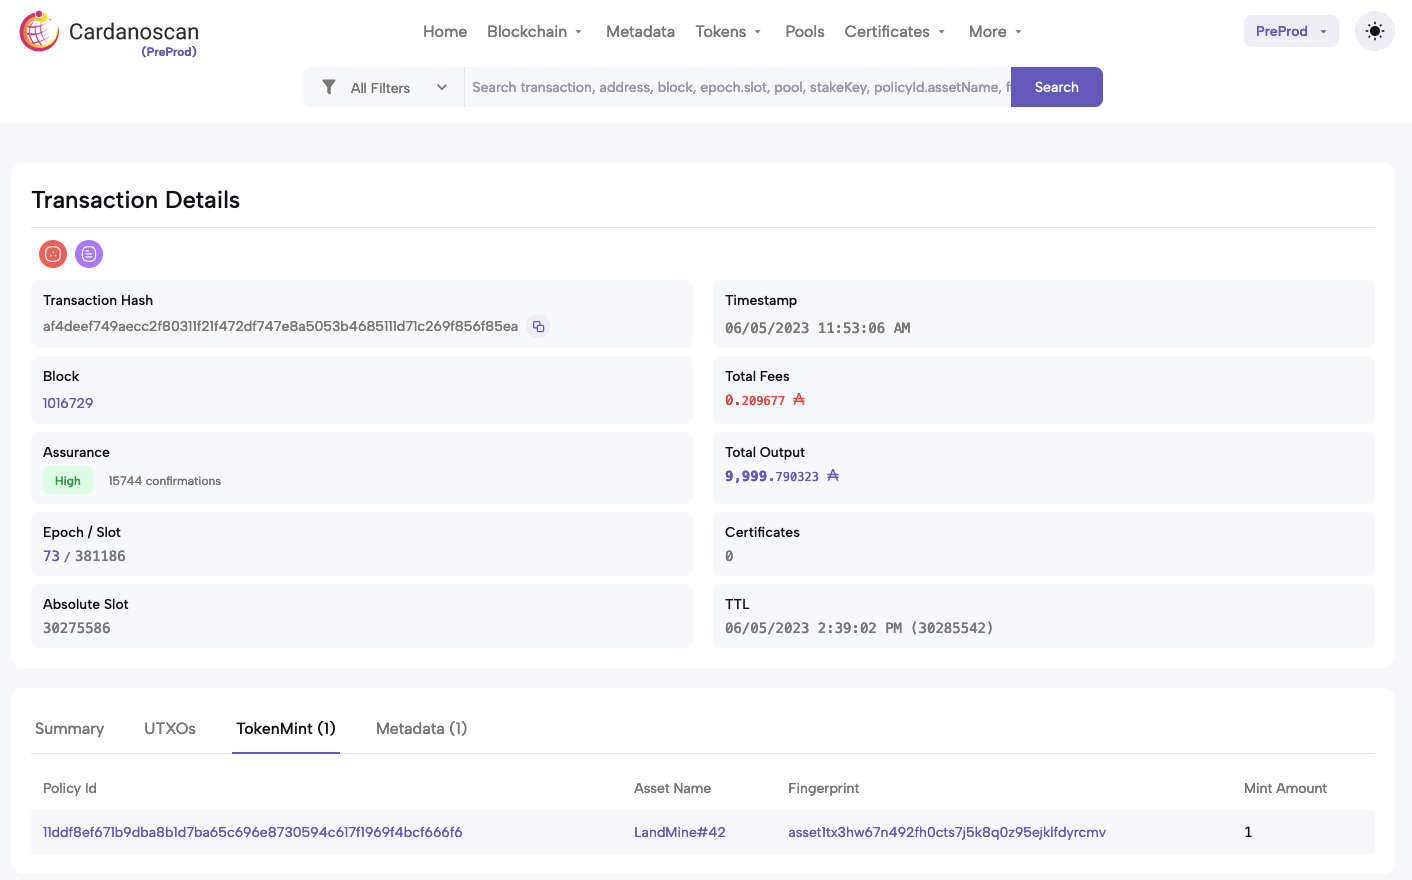
\includegraphics[width=\linewidth]{img/result-transaction.png}
\caption{Prikaz detalja transakcije na pregledniku CardanoScan}
\label{fig:result-transaction}
\end{figure}

\begin{figure}[htb]
\centering
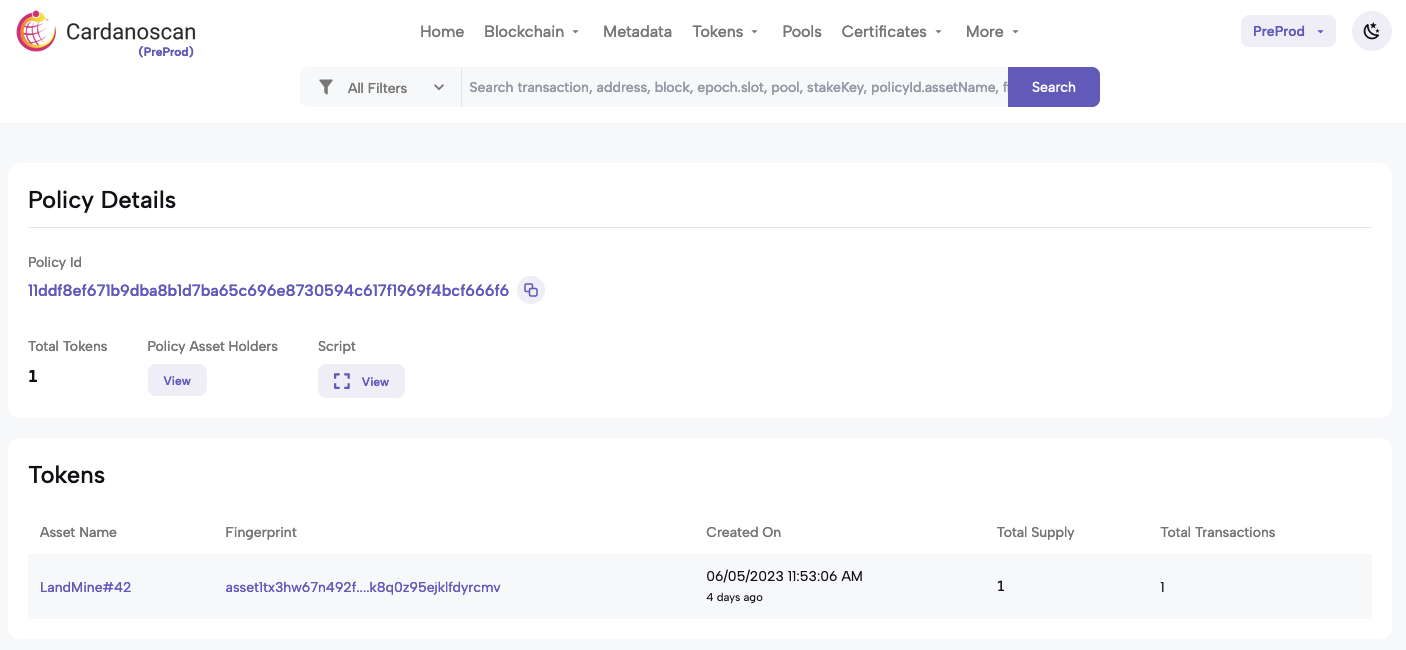
\includegraphics[width=\linewidth]{img/result-policy.png}
\caption{Prikaz politike kovanja tokena na pregledniku CardanoScan}
\label{fig:result-policy}
\end{figure}

Za pregled informacija o novom nezamjenjivom tokenu može se pretražiti transakcija \texttt{transaction\_hash} iz prethodnog koraka na pregledniku CardanoScan. Na početnom ekranu \ref{fig:result-transaction} vidljive su osnovne informacije poput sažetka transakcije, bloka u kojemu se ona nalazi, koliko blokova je naknadno nastalo, vremenska oznaka itd. Obzirom da je nezamjenjivi token usko vezan uz politiku kovanja, do istih informacija moguće je doći i pretraživanjem politike kovanja \ref{fig:result-policy}. U tom slučaju izlistavaju se svi tokeni nastali baš tom politikom kovanja, a svi dodatni detalji sadržani u tokenu vidljivi su u polju s metapodacima \ref{fig:result-metadata}.

\begin{figure}[htb]
\centering
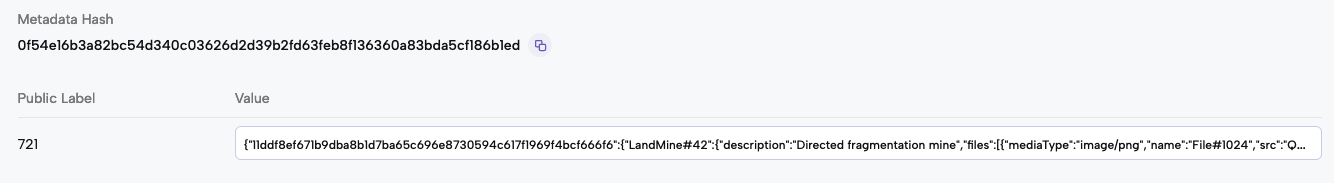
\includegraphics[width=\linewidth]{img/result-metadata.png}
\caption{Pregled metapodataka nezamjenjivog tokena na pregledniku CardanoScan}
\label{fig:result-metadata}
\end{figure}

\chapter{Zaključak}

Zaključno, tehnologija lanca blokova riješila je problem dvostruke potrošnje te tako omogućila decentralizirane transakcije s digitalnim valutama poput Bitcoina. Njezina decentralizirana priroda i transparentni sustav raspodijeljene glavne knjige promijenili su brojne industrije eliminirajući posrednike i omogućavajući konsenzus među sudionicima. Potencijalne primjene lanca blokova proširuju se na sektore kao što su upravljanje opskrbnim lancem, decentralizirane financije, zdravstvo, državne službe i prava intelektualnog vlasništva.

Jedan konkretan primjer primjene lanca blokova je u humanitarnom razminiranju koje igra ključnu ulogu u naporima obnove nakon ratnih sukoba. Korištenjem tehnologije lanca blokova, moguće je riješiti izazove povezane s pouzdanošću i sigurnosti pri pohrani osjetljivih podataka iz različitih izvora. Decentralizirana mreža čvorova osigurava pouzdanost podataka i aktora te potiče suradnju među višestrukim dionicima, poboljšavajući učinkovitost i djelotvornost operacija razminiranja.

Kao rezultat razvijeno je programsko rješenje za stvaranje nezamjenjivih tokena na lancu blokova Cardano. Takva vrsta rješenja služi kao posredna aplikacija, omogućujući drugim aplikacijama u raznim sustavima izravnu interakciju s Cardano čvorom. Korištenjem ovog rješenja, razne se aplikacije mogu neprimjetno integrirati s lancem blokova, iskorištavajući njegove prednosti dok se u isto vrijeme od njih u potpunosti apstrahiraju sve operacije vezane uz obavljanje transakcija i kriptografskih potpisa. Programsko rješenje dolazi zapakirano u Docker kontejner kako bi se eliminirala potreba za brigom o razlikama u arhitekturi, povećala razina sigurnosti i pristupa te ubrzalo skaliranje i učinkovitost potrošnje računalnih resursa.

\bibliography{literatura}
\bibliographystyle{fer}

\begin{sazetak}

Tehnologija lanca blokova transformirala je područje digitalnih valuta omogućivši decentralizirane transakcije i riješivši problem dvostruke potrošnje. Transparentna i decentralizirana priroda lanca blokova ima potencijal donijeti značajne promjene u industrijama kao što su upravljanje opskrbnim lancem, decentralizirane financije, zdravstvo, državne službe i prava intelektualnog vlasništva. U području humanitarnoga razminiranja osigurava pouzdanost i sigurnost podataka koji mogu dolaziti iz raznih izvora. Kako bi se olakšala integracija s Cardano čvorom, razvijeno je programsko rješenje koje omogućuje stvaranje nezamjenjivih tokena na Cardano lancu blokova. Takvo rješenje služi kao posrednik između drugih aplikacija i Cardano lanca blokova te pojednostavljuje složene transakcijske procese i kriptografske potpise. Kako bi se osigurala kompatibilnost, sigurnost, skalabilnost i učinkovitost korištenja resursa, aplikacija je zapakirana u Docker kontejner. Utjecaj lanca blokova obuhvaća više sektora, nudeći decentralizirana i transparentna rješenja koja potiču inovacije i poboljšavaju operativnu učinkovitost.

\kljucnerijeci{lanac blokova; Cardano; nezamjenjivi token; NFT; dokaz o udjelu}
\end{sazetak}

\newpage

\engtitle{Non-fungible tokens based on Cardano blockchain}
\begin{abstract}

Blockchain technology has transformed the field of digital currencies by enabling decentralized transactions and solving the problem of double spending. The transparent and decentralized nature of blockchain has the potential to bring about significant change in industries such as supply chain management, decentralized finance, healthcare, government services and intellectual property rights. In the field of humanitarian demining, it ensures the reliability and security of data that can come from various sources. In order to facilitate the integration with the Cardano node, a software solution was developed that enables the creation of non-fungible tokens on the Cardano blockchain. Such a solution serves as a middleware between other applications and the Cardano blockchain and simplifies complex transaction processes and cryptographic signatures. In order to ensure compatibility, security, scalability and efficient use of resources, the application is packaged in a Docker container. Blockchain's impact spans multiple sectors, offering decentralized and transparent solutions that drive innovation and improve operational efficiency.

\keywords{blockchain; Cardano; non-fungible token; NFT; proof-of-stake}
\end{abstract}

\end{document}
